% !TEX root =single_chapter_dalek.tex
\chapter{Automatic fitting of optical Type Ia Supernova spectra - the Dalek code}
\label{chap:dalek}

The last chapters (Chapters \ref{chap:sn1572_starg, chap:sn1572_hires, chap:sn1006_flames}) were dedicated to the hunt for donor stars and did not use the measurements from the \sneia themselves. In this chapter we will describe the extraction of yields and energies from optical spectra as well as the automation of this process.

The two main sources of information in spectra, are the spectra themselves as well as their time evolution. There have been a few attempts to extract the details of the stellar explosions from one or two of these sources. All of them employ the technique of fitting the spectra using synthetic spectra. One of the main parts is the radiative transfer program that creates the synthetic spectra. There are several different radiative transfer-codes in the community. 


\cite{2000PhDT.........6F} wrote a very simple radiative transfer code called \synow. \synow\ is a highly parametrized code and thus is mainly used for line identification rather than actual fitting of \snia spectra. 
The main code used in this work is a further development of the code described in  \citet{1993A&A...279..447M}  and \citet{2000A&A...363..705M}, henceforth named the \mlc. Compared to the \synow-code the \mlc-code calculates a radiative equilibrium temperature and uses this to compute internally consistent ionization ratios. In addition \mlc\ takes electron scattering into account as well as allowing for photon branching. 


Codes such as PHOENIX \cite{1999JCoAM.109...41H}, SEDONA \cite{2006ApJ...651..366K} and ARTIS \cite{2009MNRAS.398.1809K} are powerful 3D radiative transfer codes. They are the most ``physical'' codes available but take hours to days on supercomputers to produce spectra. These codes, however, are not feasible for fitting many observed spectra as they take too long for each iteration. 

The main aim of this work is to automatically fit the torrent of observed spectra expected from the current and next generation of supernova searches. We opted to use the \mlc-code as it provides a good compromise between speed and physical "realism". 

In section \ref{sec:mlc_intro} we will introduce a the inner-workings of the \mlc-code.  We will discuss the properties of the parameter space on one example fit in \ref{manual_sneia}. Section \ref{sec:ga_intro} is meant as an introduction to genetic algorithms (henceforth \ga), which are the optimization strategies of choice in the automatization of the \mlc.  We will present the current implementation of the autofitting code in Section \ref{sec:geneticdalek}. We have named the code Dalek for no particular reason. Finally we will conclude and give an outlook over future work of this unfinished project in section \ref{sec:dalek_conclusion}.

\section{The \mlc-Code}
\label{sec:mlc_intro}
As described in Section \ref{sec:intro_sn_spectra} the supernova can be divided in two different phases: the photospheric phase and the nebular phase. The \mlc-code only creates synthetic spectra for \snia\ in the photospheric phase.
In this photospheric phase the supernova is treated like a sharp photosphere emitting a black-body spectrum with a fast moving ejecta-layer on top.

\subsection{Radiative Transfer}
Radiative transfer calculations can be described as the aim to find the wavelength dependent attenuation of a given input Flux $F_0$. This wavelength dependant attenuation factor is called the opacity $\tau$:
\[
	F(\lambda) = F_0(\lambda)\,e^{-\tau(\lambda)},
\]
where $F$ is the observed Flux and $F_0$ is an assumed distribution of input flux before being reprocessed by a plasma which imposes the attenuation factor $e^{-\tau}$.
There are many physical processes in supernova radiative transfer. Of those the bound-free opacity has the biggest contribution to the final spectrum. In addition, Thompson scattering is thought to have an important effect in redistributing flux. As \mlc\ is required to run fast only bound-free opacity as well as Thompson scattering is implemented in the code.

Unlike stellar atmospheres in supernova ejecta one needs to consider the photon's doppler shift in relation to the surrounding medium. One major assumption that the code makes is that of the Sobolev approximation.  This means that the interaction between photon and line resonance happens only at one specific point (thus disregarding any broadening effects of the line). For example a photon in free flight from the photosphere will be able to interact with resonance lines of lower and lower frequencies. This Sobolev approximation is one important factor of making the code fast yet still reproducing the observed spectra rather well.

In addition the \mlc\ assumes the ejecta to be in homologous expansion. This means that the velocity is a linear function of the radius:
\[
	v=  r / t.
\]

Combining both the Sobolev approximation with the assumption of homologous expansion yields this relatively simple formula for line opacities:
\[
\tau_{lu} = \frac{\pi e^2}{m_e c}\, f \lambda t_{\rm exp} n_l\, \left(1 - \frac{g_l n_u}{g_u n_l}\right), 
\]
where $\tau_{lu}$ denotes the opacity going from the lower state to the upper state of an atom, $e$ is the electron charge, $m_e$ is the electron mass, f is the oscillator strength of the line, $\lambda$ denotes the wavelength, $t_\textrm{exp}$ the time since explosion, $n_x$ the number of atoms in the state x and $g_x$ is the statistical weight of the state x.

Although producing relatively good synthetic spectra, the assumptions of homologous expansion and Sobolev approximation have their caveats. In the case of homologous expansion it is thought to be a very good approximations in the first few minutes after the explosion. The main caveat for Sobolev approximation is that a line is not a delta-function, as assumed in the Sobolev approximation. If too strong bound-bound lines are close in frequency space it can lead to the first line shielding the second line. In summary for fast supernova fitting both approximations seem to still allow for a very well fitting spectrum.

We have discussed the propagation of the photons in the plasma but have not discussed the state of the plasma yet. The simplest assumption for the state one can make is local thermodynamic equilibrium (henceforth LTE). In this case the Boltzmann formula describes the level populations in a single ion:
\[
\frac{n_j}{n_{\rm ground}} = \frac{g_j}{g_{\rm ground}}\,e^{-(\epsilon_j - \epsilon_{\rm ground})/kT}
\]
Similarly we can calculate the ionization state using the Saha-equation:
\[
	\frac{N_j}{N_{j+1}} = n_e \frac{U_j(T)}{U_{j+1}(T)}\,C_I T^{-3/2} e^{\chi/kT},
\]
where $N_x$ are the total ion population with ionization state $x$, $U_x$ is the partition function for the ionization state $x$, $n_e$ is the number density of electrons, $C_I$ is a universal constant and al other symbols have their ususal meaning. As the ionization likelihood depends on the internal electronic state of the atom the partition function sums up over these different states:
\[
U_j = \sum_i g_{i,j} e^{-\frac{E_{i,j}}{kT}},
\]
where i describes the excitation states,j the ionization states and $g_{i,j}$ the statistical weight of the state $i,j$. 
The sum normally diverges slowly so one in practice just sums up until a highly excited state.

The \mlc\ uses the \textit{nebular approximation} which will calculate the excitation and ionization state of the SNe at nearly LTE cost. In this nebular approximation they introduce a dilution factor $W$. This is a purely geometrical factor. Treating the photosphere as a point source the factor would result in $W=1/r^2$ with r being the distance from the center. As the photosphere is expanded the dilution factor has a slightly more complex formula. An important point to note is that purely theoretical at the photosphere the dilution factor is 0.5.
The mean intensity for the supernova at a specific zone thus is given as:
\[
J = W B(T_R),
\]
where $T_R$ is the radiative temperature. The radiative temperature is estimated in the \mlc\ by matching the mean frequency of $B(T_R)$ with the mean frequency of the photon packets in the current zone (Wien approximation). W is chosen so that the frequency-integrated intensity matches the photon distribution. 

Using $W$ and $J$ one now can calculate the electronic and ionization states of the plasma:
\[
\frac{n_j}{n_{\rm ground}} = W \left( \frac{n_j}{n_{\rm ground}} \right) _{T_R}^{\rm LTE}
\]
and 
\[
\frac{N_j}{N_{j+1}n_e} = W \left( \frac{N_j}{N_{j+1}n_e} \right) _{T_R}^{\rm LTE}
\]
These approximations do not take into account physical processes like recombination to excited states and the influence of meta-stable levels. They do reproduce the physical state of the plasma relatively well on the other hand and allow for the fast computation of a synthetic spectrum.


\subsection{Monte Carlo radiative transfer}

The ejecta in the \mlc-code is divided into 20 concentric shells with an equal thickness in $1/r$, where r is the radius from the centre of the explosion. These shells have different abundances calculated at each shell midpoint from the well known empirical model W7 \citep{1984ApJ...286..644N}. There is a \textit{stratified} version of the code that allows for different abundances in each shell. We have opted to use the simple homogeneous version as the parameter space is very complex even for this homogeneous version. We plan to extend the automatic fitting procedure to use the stratified version at a later date. In addition, we assume a time since explosion $t_\textrm{exp}$ from the photometric maximum and a rise time estimate of 19.5 days. The photospheric velocity \vph, the bolometric luminosity \lbol and abundances for the chosen elements are the input parameters to the \mlc-code. 

The \mlc\ does not work with individual photons, but with photon packets. Each photon packet, described by  frequency and number of photons, and contains the same energy (more photons per packet in the red than in the blue). There are two ways to treat photon interaction. For a pure scattering interaction the photon packet is absorbed at a resonance frequency and then instantaneously reemitted with the same frequency as well as number of photons into a random direction. Newer versions of the \mlc (used in this work), however contain a photon branching implementation. In this case the photon packet is absorbed by the atom and has the chance to be emitted through a different transition. This transition is chosen by a weighted random process. The number of photons in the packet is adjusted to conserve the co-moving energy of the packet. Our one dimensional model is divided into multiple geometric shells.  They do have a density  Using an initial guess of \teff\ for the photosphere, one can calculate the plasma condition in each shell.

The Monte-Carlo simulation begins. A photon packet is emitted with a random frequency and a random angle drawn from a Blackbody distribution $B(T)$.  An event optical depth is calculated from a uniform random distribution so that $\tau_{\rm event}=-ln(z); z \in (0,1]$.  There are three possible outcomes for the photon in each Monte Carlo step: We calculate the length of the path ($s_e$) that the packet can travel freely before $\tau_{\rm event}$ is equal to the Thompson scattering opacity $\tau_{\rm event} = \sigma_\textrm{T} n_e s_e$. Next we calculate the same path length for the lines $s_l$ using as a target opacity $\tau_e + \tau_\textrm{line}$. If both paths are longer than the path to exit the current shell, then the photon exits the current zone and a new Monte Carlo step begins. In the case that $s_e$ is the shortest then Thompson scattering occurs and the photon is assigned a new direction and a new $\tau_\textrm{event}$ is drawn and we start anew. In the case of line scattering the excited atom can de-excite through many lines. \mlc\ randomly chooses a downward transition for the whole packet (taking the appropriate weights into account). The number of photons in the packet is adjusted to ensure that the energy is conserved in the comoving frame. 

There are two possibilities for the final fate of the photon. Either it is reabsorbed into the photosphere or is emitted from the supernova. When initializing the state of the plasma one assumes an initial guess for the photon temperature. An initializing Monte-Carlo simulation runs and records each packet status at the mid-point of each shell. This information is used to calculate a new photospheric temperature and a updated plasma conditions (level population and ionization). This procedure is repeated until the photospheric temperature converges. Once convergence is reached the actual Monte-Carlo simulation begins. 

The final spectrum is not calculated using the escaping photons. Instead we calculate the optical depths from the escaping photons and then calculate the emerging spectrum using the formal integral. 
This has the advantage of reducing noise in the spectrum due to Monte-Carlo noise and gives very good results. A more detailed description of the code can be found in  \citet{1993A&A...279..447M} and \citet{2000A&A...363..705M}.


\section{Manually fitting a Type Ia supernova}
\label{sec:manual_sneia}
When fitting manually there are several features that help guide the direction of the fit. We will attempt to explain this by using a spectrum of SN2002bo 10 days before maximum \citep{2004MNRAS.348..261B}. 
Directly measurable are the redshift of the supernova (and implied distance) and the time of the spectrum relative to maximum. We calculate the time since explosion ($t_\textrm{exp}$) using the photometric maximum and assuming a rise time of 19.5 days.
The other parameters are initialized using empirical data (see section \ref{sec:dalek}). 

\begin{figure}[htbp] %  figure placement: here, top, bottom, or page
   \centering
   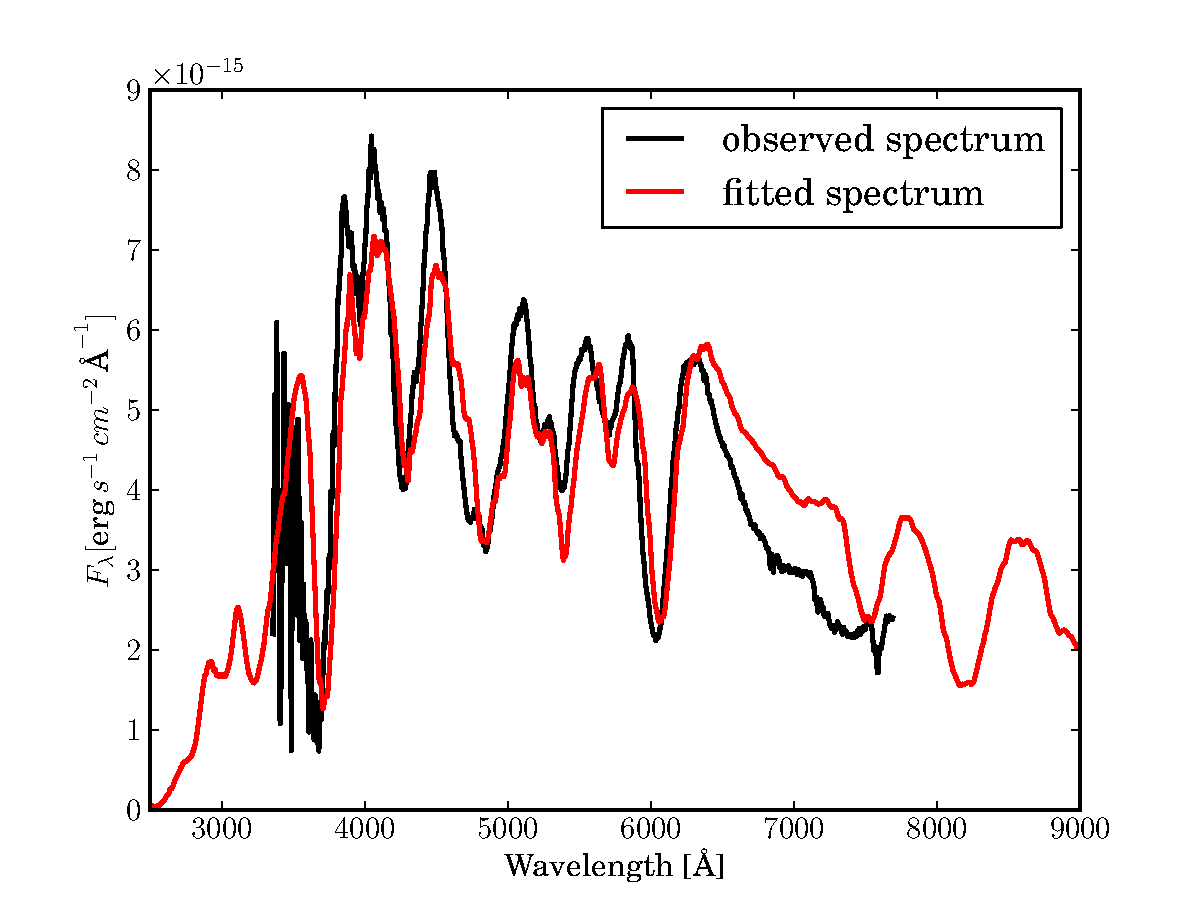
\includegraphics[width=0.7\textwidth]{chapter_dalek/plots/bf2002bo-10.pdf} 
   \caption{Spectrum of \sn{2002}{bo} \citep{2004MNRAS.348..261B} with \mlc-fit by \citet{hachinger_dipl2007}. The excess in redwards of 6500\,\AA\ is a common problematic features of these fits.}
   \label{fig:sn2002bo-10_bf}
\end{figure}

Stephan Hachinger has kindly provided his manually obtained best fitting parameters ( for the supernova at this stage (see Figure \ref{fig:sn2002bo-10_bf}).
The best fitting parameters for this spectrum are $\loglbol=9.05$ and $\vph=11700$. We have listed the non-zero abundances in Table \ref{tab:sn2002bo_perf_param}. Nickel is often given in terms of undecayed nickel ($\textrm{Ni}_0$) and will then split up into its daughter nuclei \Co and \Fe. $Fe_0$ designates the primordial iron abundance and is added to the iron abundance which results from the  nickel decay. We assume in any further discussions in this work that cobalt is always \Co and is never assumed to be stable. 

\ctable[
caption = {Abundance parameters for best fit},
	% 
	label   = {table:2002bo_bestfit_abundances},
	%
	%
]{lc}{
}{ \FL
% 
Atom & Abundance \ML
Carbon & 0.08 \% \\
Oxygen & 54.9 \% \\
Magnesium & 10 \% \\
Silicon & 25 \% \\
Sulfur & 4.5 \% \\
Calcium & 1 \% \\
Titanium & 0.01 \% \\
Chromium & 0.07 \% \\
primordial Iron & 0.07 \% \\
undecayed Nickel & 1.5 \% \\
\LL}

In Figure \ref{fig:sn2002bo-10_bf} P-Cygni profiles of many features are easily visible. The calcium line in the blue can be seen to be to blueshifted in relation to the model. This property is not unusual and is thought to come from high velocity calcium components at the outer edge of the ejecta. This can be often rectified in the stratified version of the \mlc-code. The next major known discrepancy is the excess of flux redwards of  $\approx 6200 \AA$.  This is a common problem as the wrongful assumption of an underlying black body spectrum overestimates the flux in this region. When fitting manually often one tries to fit the depth of the lines instead of the continuum.

\begin{figure}[htbp] %  figure placement: here, top, bottom, or page
   \centering
   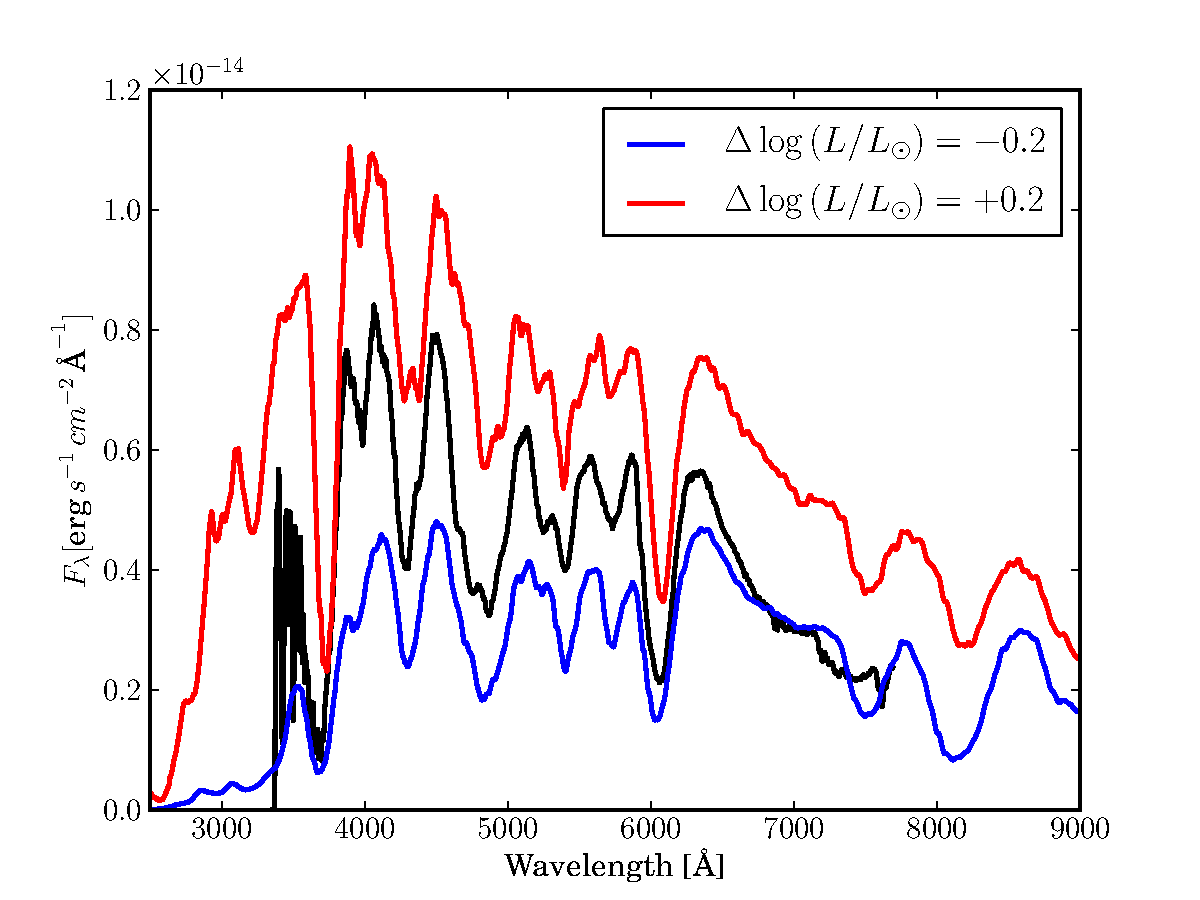
\includegraphics[width=0.7\textwidth]{chapter_dalek/plots/bf2002bo-10_lum.pdf} 
   \caption{We have perturbed the luminosity around the best fit value. The most noticeable effect is the continuum offset. There is also a slight change in the overall slope of the spectrum.} 
   \label{fig:sn2002bo_lum_offset}
\end{figure}

There are three main parameters that have the most influence on the overall spectrum fit: Luminosity, photospheric velocity and abundance in iron group elements.
A large offset in \lum\ to the best fit parameter is easily visible as a large offset of the continuum (see Figure \ref{fig:sn2002bo_lum_offset}. Thus it is easy to constrain the parameter space in \lum. \lum\ also has influence on the temperature of the model through:
\[
L_{\rm bol} = 4\pi\sigma\, R^2\,T^4 = 4\pi\sigma\,\vph\,\texp.
\label{eq:lum_temp_relation}
\]

Velocity in astronomy is often measured using the doppler shift of atomic lines. In this case however it is hard to measure the photospheric velocity from atomic lines.  Lines are created at different depths and thus at different velocities. This smears out the line profiles which makes fitting velocities nearly impossible using this technique. The main impact of photospheric velocity is establishing the temperature structure with the given luminosity. A model with a too high photospheric velocity will have expanded more than the observed spectrum and thus will be cooler. This results in a spectrum that is too luminous in the red and not luminous enough in the blue (see Figure \ref{fig:sn2002bo_vph_offset}). 
A secondary effect is that the ion population will be off. This can be determined by judging the fit of \ion{Si}{2} lines versus the fit of \ion{Si}{3} lines. 
\begin{figure}[htbp] %  figure placement: here, top, bottom, or page
   \centering
   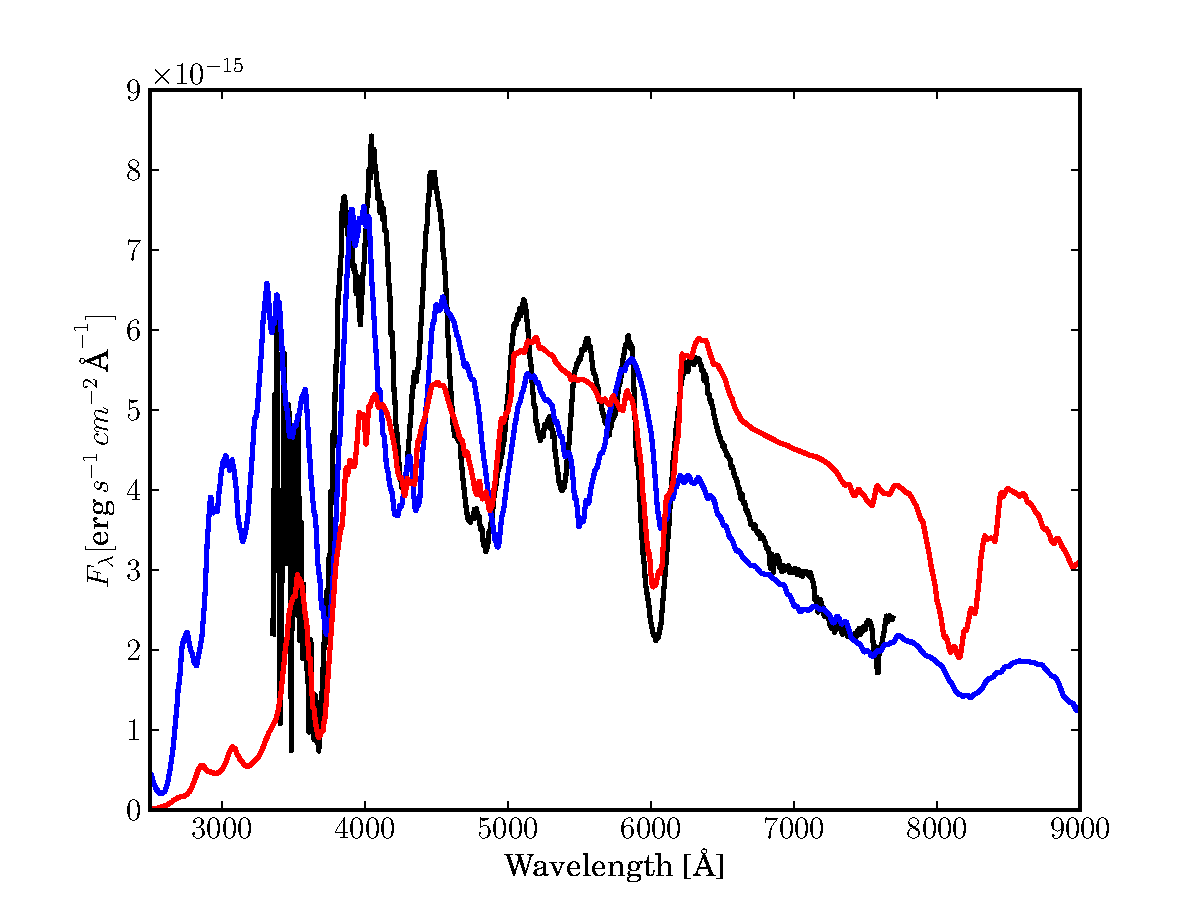
\includegraphics[width=0.7\textwidth]{chapter_dalek/plots/bf2002bo-10_vph.pdf} 
   \caption{The photospheric velocity has been perturbed around the bestfit. The slope of the spectrum changes a too small velocity produces a hot blue spectrum, a too large velocity a cold red spectrum.}
   \label{fig:sn2002bo_vph_offset}
\end{figure}


The initial abundances for each fit are determined by integrating the abundances above the photosphere in the W7 model \citep{1984ApJ...286..644N}.

The \ige\ have a similar influence on the overall flux distribution as the photospheric velocity. 
We assume, as discussed previously, no stable Cobalt. The input parameters for Nickel, Cobalt and Iron are the undecayed $\Ni_0$ and the primordial $\Fe_0$. We use the time since explosion to calculate the abundances using radioactive decay. The other important \ige s are Titanium and Chromium which have no easily identifiable single lines in the observed spectra.  All \ige\ elements reprocess the flux heavily by absorbing in the bluewards of $\approx 3800\,\AA$ and fluoresce in the red part of the spectrum. For example, a too high abundance will suppress the flux in the blue too much and will cause the spectrum to be over-luminous in the red (see Figure \ref{fig:sn2002_ige_offset}). Although physically different from the photospheric velocity, phenomenologically these are similar. The degeneracy is broken by identifiable Fe-Lines in the red part of the spectrum as well as the ionization balance determined by the temperature (mainly influenced by photospheric velocity and luminosity). This near degeneracy causes a very complex parameter space. We disregard the elements Scandium, Vanadium and  Manganese as they seem to have little influence on the spectrum at their predicted abundances.

\begin{figure}[htbp] %  figure placement: here, top, bottom, or page
   \centering
   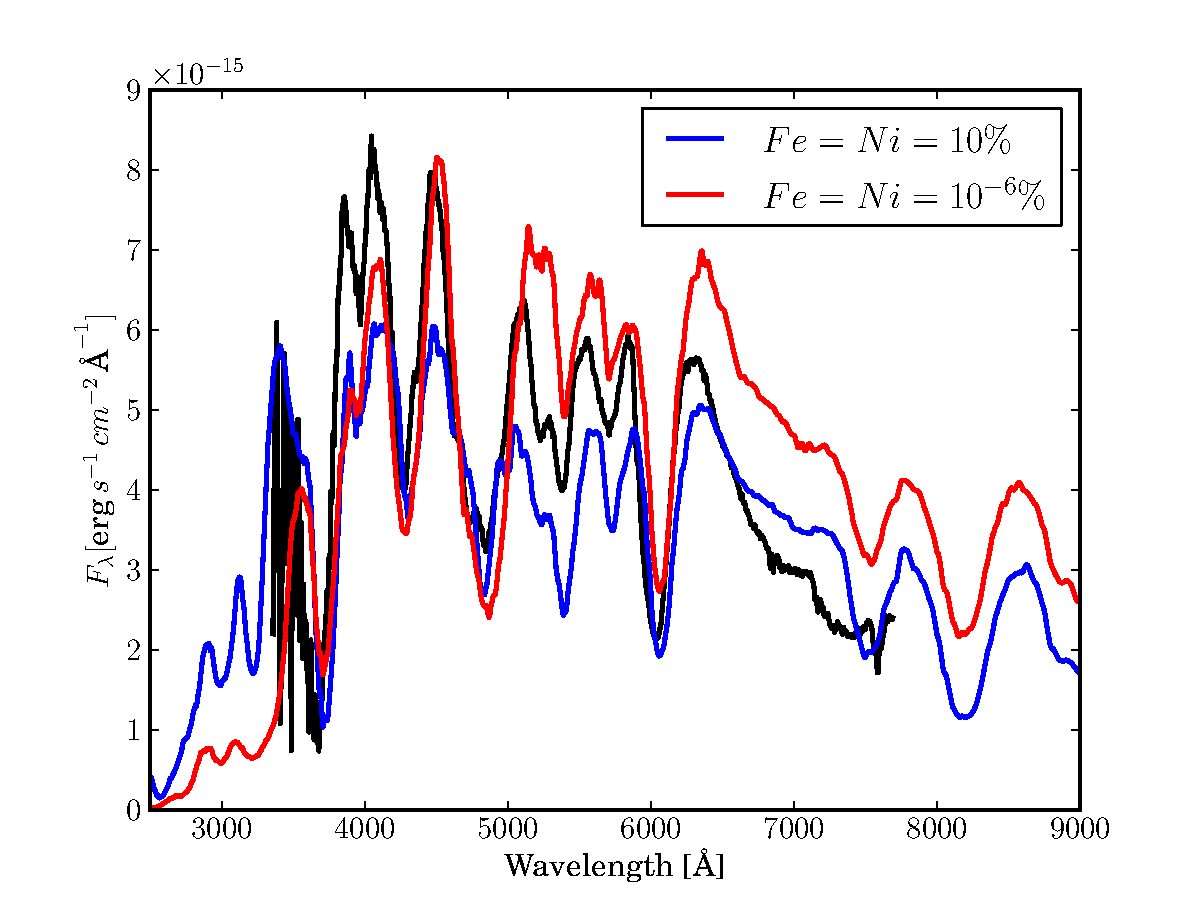
\includegraphics[width=0.7\textwidth]{chapter_dalek/plots/bf2002bo-10_ige.pdf} 
   \caption{When changing the \ige\ (in this case we have only changed iron and Nickel) the flux is altered in the blue and red part. Too much \ige s and there's not enough flux in the blue and too much flux in the red and vice versa.}
   \label{fig:sn2002bo_ige_offset}
\end{figure}

There are six other abundances that are taken into account when fitting: Carbon, Oxygen, Magnesium, Silicon, Sulfur and Calcium (see Figure \ref{fig:sn2002bo_lineident}). Oxygen does not have lines except the Oxygen triplet at 7778 \AA and plays a special role in the fitting process. Oxygen acts as a buffer element and is assigned the remaining fraction that is left after all elements have been given abundances. We do acknowledge that this might physically not be correct and a change in the density structure would be more appropriate. This, however would introduce an additional free parameter and make fits much more complex.

Judging the fit of the \ion{Ca}{2} line at 3700\,\AA is relatively easy and thus the calcium abundance is usually changed first. Additionally, the choice of temperature imposed by photospheric velocity and luminosity does not have an immense influence on this line. One caveat however is that the \ion{Ca}{2} line saturates at a certain abundance. If the observed \ion{Ca}{2} line is close to that limit one can only extract a lower limit for Calcium.
Silicon and Sulfur are usually the next elements to be fine-tuned. Both of these elements are linked through nuclear synthesis and we don't expect there to be more Sulfur than Silicon. We also expect no less Sulfur than a third of Silicon. Silicon also provides an important measure for temperature through the ionization balance of \ion{Si}{2} to \ion{Si}{3} (see Figure \ref{fig:sn2002bo_lineident}). The strong strong \ion{Mg}{2} feature near 4300 \AA helps constrains the Magnesium abundance. The weak \ion{C}{2} feature at $\approx 6300\,\AA$ is the only line to provide constraints for the carbon abundance. In most \sneia-spectra this line is weak or not visible.
\begin{figure}[htbp] %  figure placement: here, top, bottom, or page
   \centering
   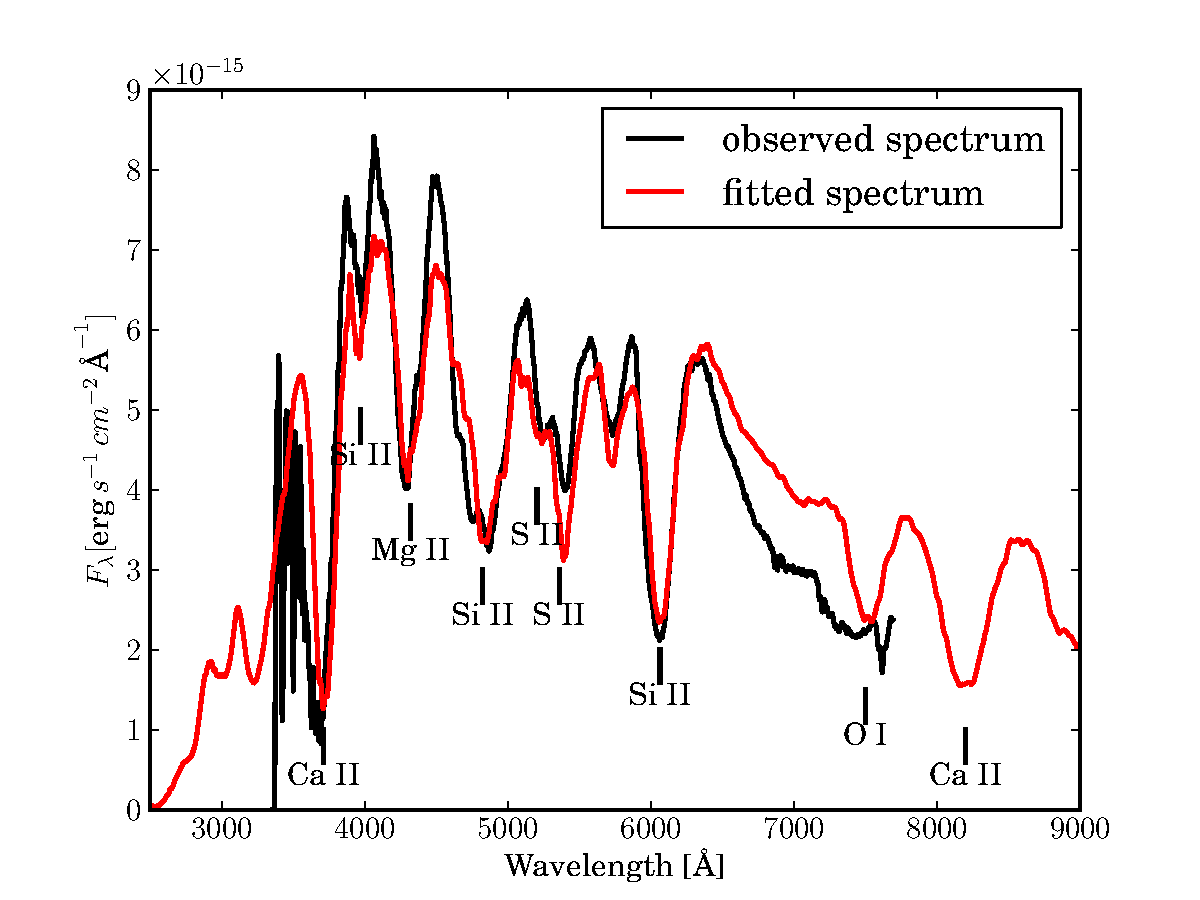
\includegraphics[width=0.7\textwidth]{chapter_dalek/plots/bf2002bo-10_lineid.pdf} 
   \caption{We have identified some of the strongest lines that are scrutinized when fitting a \sneia\ spectrum.}
   \label{fig:sn2002bo_lineident}
\end{figure}

The fitting process involves first adjusting luminosity and then \ige s as well as photospheric velocity. This is followed by adjusting the other elemental abundances from the initial W7 values \citep{1984ApJ...286..644N}. After the elemental abundances are adjusted we re-adjust the luminosity, photospheric velocity and \ige. This iterative process continues until a satisfactory fit has been obtained. When closing in on the optimal fit we do observe the dilution factor. Purely theoretical we would expect this to be close to 0.5 for a ``physical'' fit. We do, however accept values between 0.4 and 0.7 as physical. This large range is accepted due to numerical fluctuation and approximations made by the \mlc. The parameters are often improved further by checking their time evolution through fits of photospheric spectra at different times.


In summary, the fitting of a supernova is a complex procedure and requires a lot of practice. For automating this process we initially tested simple gradient methods. These failed abysmally. We quickly discovered the search space is too complex and evaluation time takes too long (each synthetic spectrum roughly one minute on a modern computer) to use these simple methods. Research in numerical optimization techniques haa made significant process in the last decades. These areas of mathematics have yielded impressive algorithms. Genetic algorithms are easy to implement and are intrinsically parallel. A perfect match for our problem.

 
\section{Genetic Algorithms}
\label{sec:intro_ga}

Finding optimal solutions in complex search spaces is one of the main fields in numerical mathematics.  They have wide ranging applications in engineering, bio sciences and physical sciences. There have been several immense advances in optimization algorithms over the last decades.
Among them is the  remarkable feat of quickly finding solutions for famous traveling salesman problem with simulated annealing \citep{Kirkpatrick13051983} and later with ant colony optimization \citep{Dorigo97antcolonies}.

Another major accomplishment was the development of evolutionary algorithms and subsequently genetic algorithms. The idea of an algorithm which imitates the principal of natural evolution was first introduced by \cite{Holland:1962:OLT:321127.321128}. These evolutionary algorithms have since become a sizeable subfield of numerical optimization. Genetic algorithms (henceforth \ga), a subclass of evolutionary algorithms, were further developed by John Holland's student David Goldberg.  \citep{citeulike:125978} is the standard textbook for \ga s.

Optimization algorithms have two seemingly conflicting goals: exploiting good leads (optimum seeking) while still exploring the parameter space sufficiently. Simple algorithms like Hillclimbing (randomly selecting a point in the neighbourhood of the current point and then picking the more optimal point as the new basis) will exploit good leads but will neglect to explore the search space leading to the convergence on local optima. This often leads to be stuck at extrema. Whereas random searches are excellent at exploring the search space but will fail to quickly converge on an optimal solution. Which algorithm to use, naturally depends on the type of parameter space. Spaces with independent variables can be solved relatively simply by employing optimum seeking methods. Random search algorithms are suited to parameter spaces with highly co-dependant variables. Genetic algorithms do strike a balance between exploration and exploiting the current best solution. Consequently they can be applied to a wide range of different parameter spaces.

Genetic algorithms are a heuristic search technique to find optimal solutions in n-dimensional search spaces. Generally in optimization we consider the function $f(\vec{x})$ with the multi-dimensional solution $\vec{y}$. In addition, we define a figure-of-merit function $g(\vec{y})=s$ where s is a scalar. It is the goal to find the input vector $\vec{x}$  to maximize or minimize $s$. In \ga s a single solution ($\vec{x}$) is called an individual (sometimes also referred to as a genome). The individual components of the vector $\vec{x}$ are referred to as the genes. We also differentiate between the vector representation called genotype, and the solution vector for an individual ($\vec{y}$ using the previous notation) called phenotype. This is similar to biology where the input $\vec{x}$ can be thought of as the DNA sequence. The phenotype in biology however does not resemble a vector.  Mathematically speaking it is possible to have multiple genotypes map to one phenotype, however each genotype only maps to one phenotype. The figure-of-merit function $g(\vec{y})=s$ is often referred to as the fitness function. 
Following the notation of \citep{Michalewicz:1994:GAD:184675} we introduce the population $P(t)$ with the individuals (sometimes referred to as genomes) $\{p_{1}^{t}, \dots, p_{n}^{t}\}$, where $t$ denotes the iteration (also called generation). Each individual $(p_{i}^t)$ is a data structure consisting of a vector $\vec{x}_i$ and its corresponding fitness scalar $s_i$.  When we speak of evaluating $p_{i}^{t}$ we mean that we use $g(f(\vec{x}_i))=s_i$ to determine the fitness. A new population (or generation) $P(t+1)$ is formed by choosing,  in the \textit{select step}, the more fit individuals. Some or all of the new population undergo transformations in the \textit{recombine step}. Generically these transformations are called genetic operators. We define unary transformations, which create new individuals by small changes in single individuals called mutations. Higher order transformations called crossovers combine the traits of multiple individuals to form a next generation individual. 
After the new population has been created in the \textit{recombine step}, it is evaluated (perform the computation $g(f(\vec{x}_i))=s_i$) and the \textit{select step} begins anew. 

This procedure is repeated until the best individual has reached a certain threshold fitness (see Algorithm \ref{alg:evol_program}). 



\begin{algorithm}
\label{alg:evol_program}
\caption{Structure of a genetic algorithm}
\begin{algorithmic}
\STATE $t \gets 0$\\
initialize $P(t)$\\
evaluate $P(t)$
\WHILE{(\textbf{not} termination condition)}
\STATE $t \gets t+1$\\
select $P(t)$ from $P(t-1)$\\
recombine $P(t)$\\
evaluate $P(t)$
\ENDWHILE
\end{algorithmic}
\end{algorithm}

An optimization problem needs to have the following traits to be solvable by a \ga:
\begin{itemize}
\item a genetic representation of the search space (e.g. a vector)
\item a function (or a chain of functions) that can calculate a fitness for a genetic representation
\item transformations that create a new population/generation out of selected members of the old population/generation
\item a method of creating an initial population
\end{itemize}


If the problem fulfills all these requirements one can start constructing a \ga. This involves multiple steps the first of which is choosing a suitable genetic representation for each solution in the parameter space. 

\paragraph{Genetic Representation:}
There are two main ways to represent a genome: binary encoding and value encoding (sometimes called gray encoding). Binary encoding was the form of encoding  used in early genetic algorithms. It offers significant advantages when trying to optimize very simple problems. In one-dimensional problems, for example, value encoding only offers one gene, whereas binary encoding, depending on the requested precision of the value, offers multiple genes. This becomes obvious in the one-dimensional minimization xample: $f(\vec{x})=(x_0 - 3.141)^2$. The solution vector that minimizes the problem in value encoding is $\vec{x} = (3.141)$ using IEEE 754 floating point encoding the optimal vector is $\vec{x}=(0,1,0,0,0,0,0,0,0,1,0,0,1,0,0,1,0,0,0,0,0,1,1,0,0,0,1,0,0,1,0,1)$.
There are however many problems with binary encoding. The so called \textit{hamming cliff} describes the problem that a simple bit-flip at one high encoding bit (occurring in some genetic operators like mutation) can dramatically change the encoded value \citep[e.g.][]{Chakraborty2003253}. This can improve covering of search space but also can hinder the code from converging. When using binary encoding for many input variables the genomes can get incredibly long. \ga s have been shown to perform poorly for very long genomes. Value encoding often is a natural way to encode the parameters of a problem. In contrast to binary encoding the genetic operators are often much more problem specific. It seems that for the moment value encoding is the preferred method in many cases \citep[e.g.][]{Janikow1991Comparison,Wright91geneticalgorithms,Goldberg90real-codedgenetic}

Finally, an important encoding to mention is that of permutation encoding. In the famous case of the travelling salesman problem (henceforth \tsp) one tries to find the shortest route between n cities. In this case each city can only be visited once and the route must end in the starting city. There are many algorithms that can solve this problem. Brute force attempts scale with $O(n!)$ which make them unfeasible. A genetic algorithm can solve this problem by encoding the order (permutation encoding) in which the cities are visited in each genome. There are special genetic operators for permutation encoding. For the \tsp\ there are better algorithms like dynamic programming which can solve the problem with a complexity of $O(n^2 2^n)$ (see Figure \ref{fig:xkcd_tsp}).

\begin{figure}[htbp] %  figure placement: here, top, bottom, or page
   \centering
   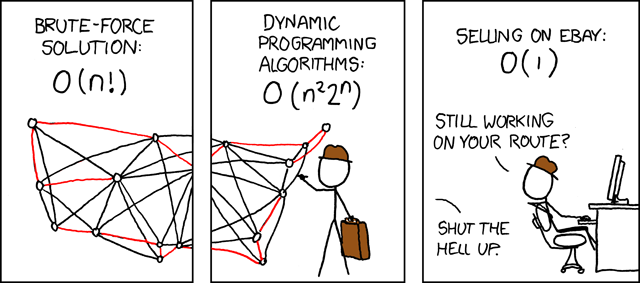
\includegraphics[width=0.7\textwidth]{chapter_dalek/plots/travelling_salesman_problem.png} 
   \caption{The death of the \tsp\ with the advent of online sales. (reproduced with kind permission by xkcd.com)}
   \label{fig:xkcd_tsp}
\end{figure}



The fitness function maps the phenotype ($\vec{y}$) to a scalar. Fitness functions are very problem dependent and are often hard to define. It might not always be possible to find a function that maps desirability to exactley one value (e.g. it is not possible to map desirable traits of a car to one number and optimize that). This class of problem is generally referred to as multi-objective optimization and is an active field in \ga-research \citep{citeulike:1300532}. Describing this subfield is outside the scope of this work. A \ga\ is required to follow promising leads but also explore the parameter space. It sometimes happens that a fitness function values a small fraction of individuals extremely high when compared to the rest of the solutions. This can become a problem when this high fitness value is only tied to a few genes. For example, a right value of the first gene could cause much higher fitness then correct values of other genes in a single individual. The subsequent populations will then be reigned by the genes of this one individual which prohibits the \ga\ to explore the search space.  In \ga-terms individuals with extremely high fitness based on very few gebes are called "superindividuals". They can drastically reduce the genetic breadth and often cause the \ga to fail. One way to overcome this problem is scaling the fitness of all individuals after they have been computed. There are other steps which can be undertaken in the \textit{select step} described later. The scaling is often a simple algebraic transformation, like linear or exponential scaling. The coefficients for this transformation are often calculated by using the average, minimal and maximal value of the fitness distribution. A specific example can be found in Section \ref{sec:geneticdalek}. In summary, fitness functions and scaling are a very crucial part of a successful algorithm. For a description of different scaling methods please refer to \citet{Kreinovich93geneticalgorithms}.

The most basic quantity to consider when choosing the initial population is that of population size. Generally the population size remains the same over the course of a \ga. The population size should be chosen in relation to the size of the parameter space. A small population size and a large search space can lead the \ga\ to find local optima rather than the global optimum. We have in our work chosen a population which is roughly 15 times bigger than the number of genes. After having chosen the population size the most basic method of selecting the initial population is to draw individuals uniformly and randomly from the entire search space. One might however know a probability distribution for the parameter space and can draw randomly weighted by the distribution (e.g. when trying to find find parameters for a random star, we can rule a 20\,\msun white dwarf with some likelihood). An initial population that is closer to predicted optimal value will converge faster, but won't explore the parameter space that well. 

Once we have evaluated the fitness for each member of the individual population the next step is the \textit{selection step}. There are many different approaches for selecting individuals from the current population to create the next population. Before selecting individuals we can make coarse selection on the entire population. One selection that is often performed is \textit{elitism} in which a fraction of the fittest individuals is selected to advance unaltered to the next generation. On the other hand one can discard a fraction of the least fit individuals. These discarded individuals (including their gene-combinations) won't be used in the recombination step. The remaining population is called the mating population.

After we have performed a coarse selection on the population we start with the recombination step. The first action in the recombination step is the selection of two or more individuals from the mating population and add them to a mating pool. In all our next examples we will assume a mating-pool with only two slots (similar to two parents in biological reproduction). Once the mating pool is filled a new individual is created by combining the genetic information of all members in the mating pool. There is a multitude of options for selecting members from the mating population and adding them to a mating pool \citep[for an overview see]{Goldberg91acomparative}. The most widely used of the selection algorithms is \textit{roulette wheel selection} (see Figure \ref{fig:roulettewheel}). \textit{Roulette wheel selection} is in the class of \textit{fitness proportional selection}. In addition to \textit{fitness proportional selection} there is \textit{rank selection}. In rank selection the fitness only influences the rank of the individuals (see Figure \ref{fig:rankselection}). The previous described fitness scaling and rank selection have similar effects. They do alleviate the problem of ``super-individuals'' that will dominate the following generations and often lead to the failure of the \ga. Finally, in \textit{tournament selection} we randomly select two individuals and compare those. The fitter of those two individuals is selected and added to the mating pool. 

There are multiple steps for creating a new population from the current mating population. First we select two individuals (or more) using our selection process (e.g. \textit{roulette wheel selection}) and place them in a mating pool. The reader should notice that the same individual can be in the mating pool twice! We create one or multiple new individuals (children) from this mating pool and place them in the new population (also known as the next generation). The current mating pool is disbanded and a new one is formed. These steps are repeated until the new population has the same number as the old population (minus the number of individuals that automatically advanced to the new population through \textit{elitism}). 
There are two main processes to create a new individual from a mating pool: crossover and mutation.
\begin{figure}[htbp] %  figure placement: here, top, bottom, or page
   \centering
   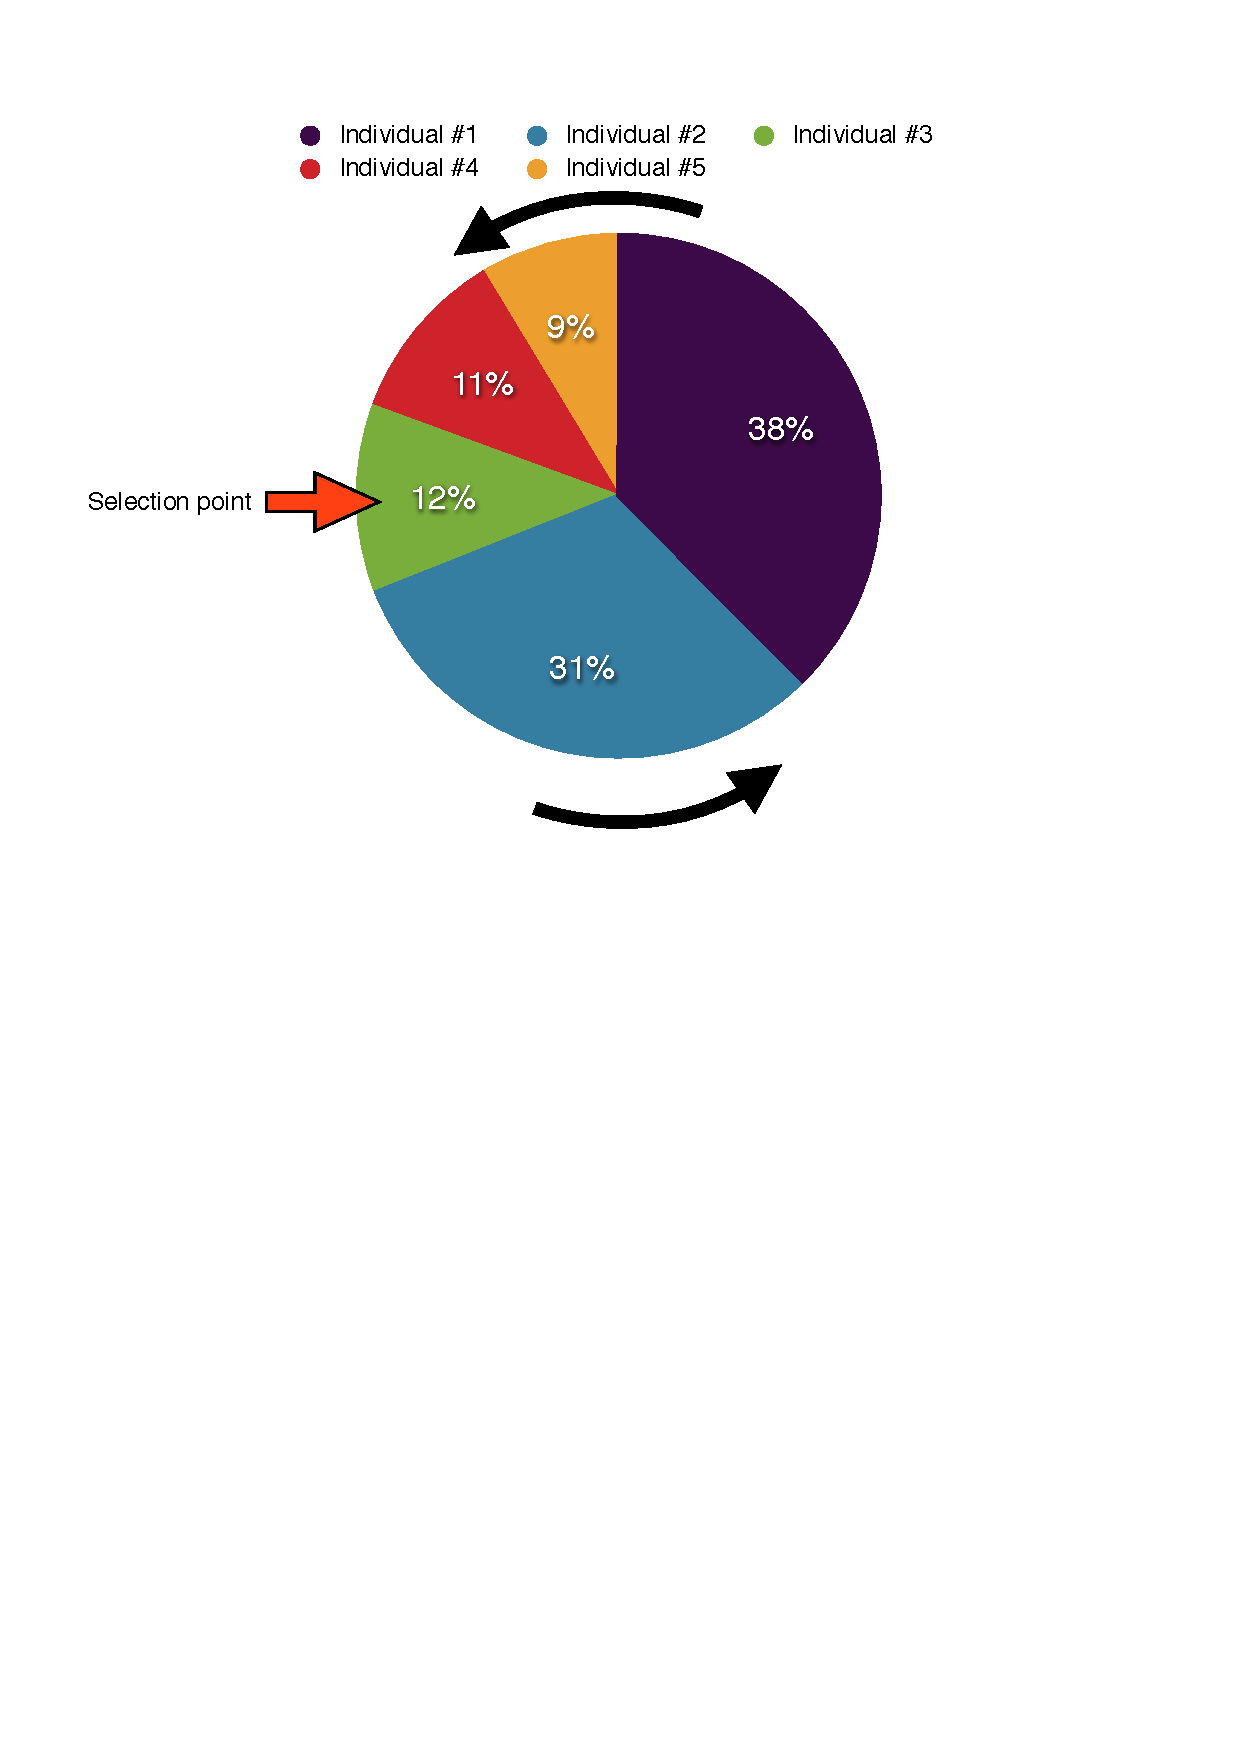
\includegraphics[width=0.7\textwidth]{chapter_dalek/plots/rws_cropped.pdf} 
   \caption{The individual fitnesses are assigned proportional fractions on the roulette wheel. The wheel is then spun and will slowly decelerate and stop at some point. Individuals with a higher fitness have a higher chance of being chosen with this method.}
   \label{fig:roulettewheel}
\end{figure}

\begin{figure}[htbp] %  figure placement: here, top, bottom, or page
   \centering
   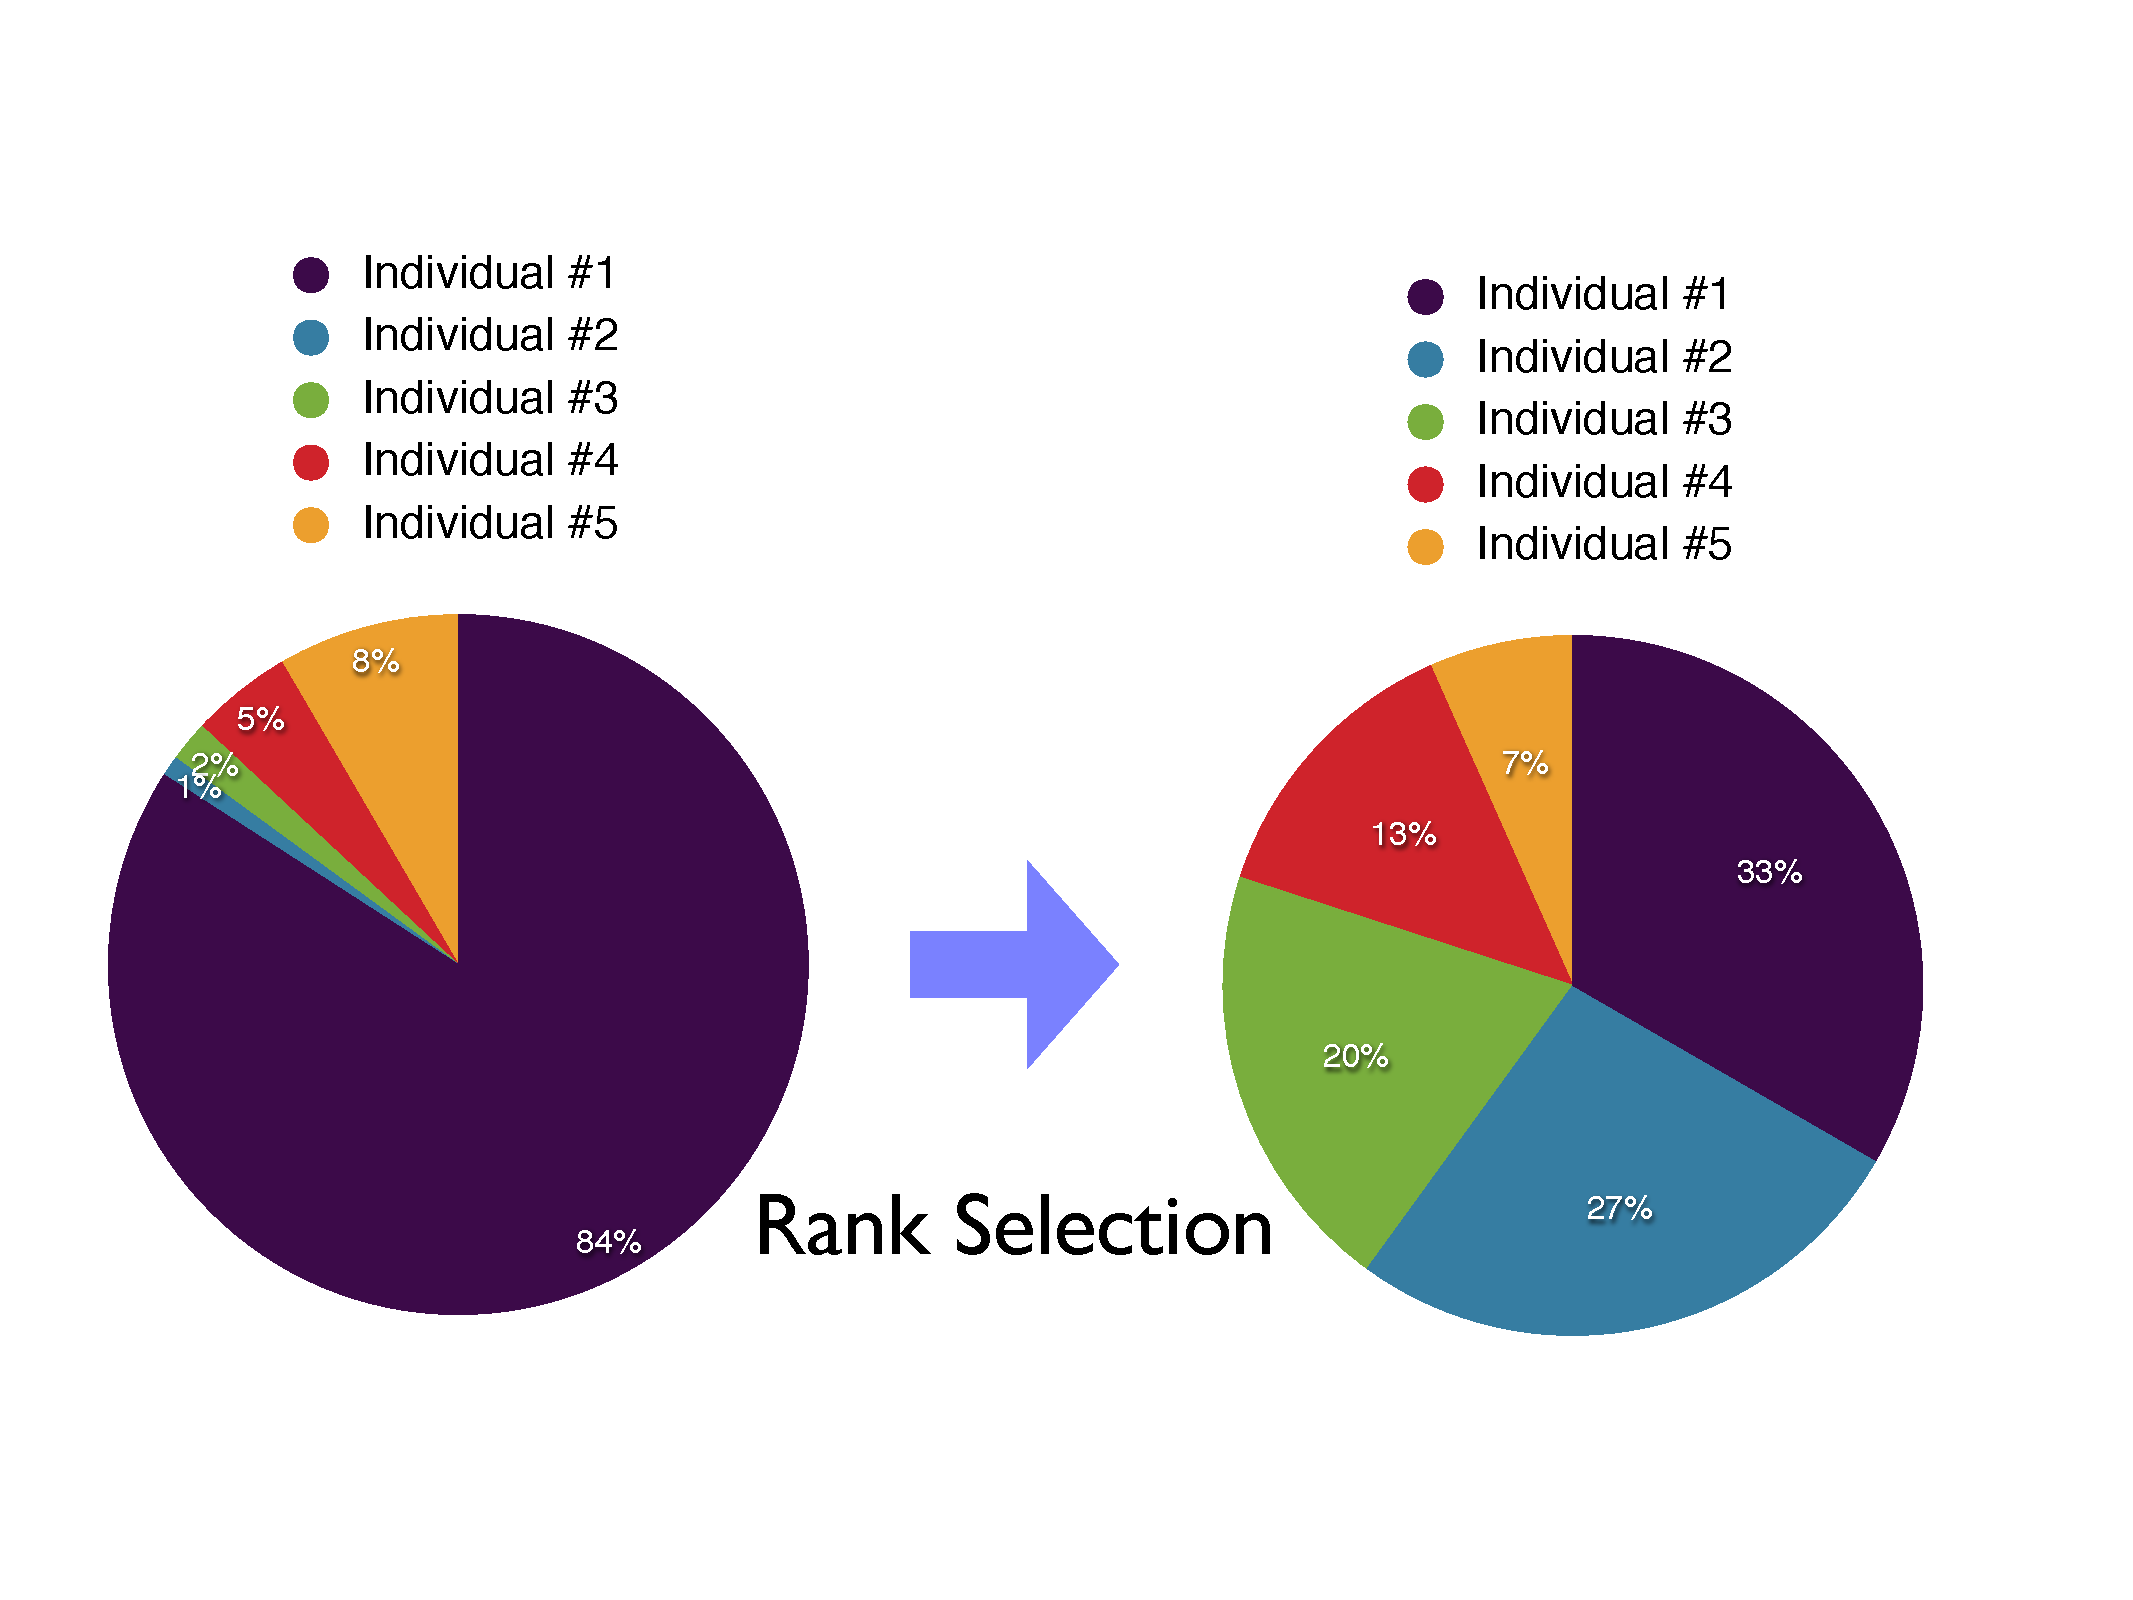
\includegraphics[width=0.7\textwidth]{chapter_dalek/plots/rank_select.pdf} 
   \caption{We assign new fitness values to individuals before assigning them probabilities on the roulette wheel. The fitnesses are assigned by location in an ordered list. The least fit individual gets assigned the value 1 the fittest individual the number n, where n is the population size. This is can be viewed as a special case of fitness scaling. After the new fitnesses have been chosen we use normal roulette wheel selection to select for the mating pool in the population. }
   \label{fig:rankselection}
\end{figure}

To describe these two options in detail we assume a mating pool with two individuals. The simplest form of a crossover is the single-point crossover (see Figure \ref{fig:crossover}). A random integer $r \in [1,N-1]$, where N describes the number of genes per genome is selected. The new individual is created out of the first $r$ genes from the first parent and the last $N-r$ genes from the second parent. Now it is trivial to create a second child (using the same random number $r$) from the mating pool by just switching first and second parent. 
Two-point crossover is very similar to single-point crossover. Two random numbers are selected and the crossover occurs at these places. Multi-point (see Figure \ref{fig:crossover}) is essentially just a extrapolation of two point crossover. Finally, there is uniform cross-over in the case that each gene is selected randomly with equal chance from either parent.
Arithmetic crossovers use a function to calculate the new gene from each of the parent genes. For a value encoding this function could be the mean. For a binary encoding the function could be the \textit{and} operator. ???should I include example???
One can mix arithmetic and binary crossovers. For example we select the $r$ genes from the first parent and create the last $N-r$ genes by taking the mean of first and second parents' genes. 
After the new child or children have been created through crossovers they are subjected to the mutation operator. There is a chance for each individual gene (often chosen to be less than 5\%) that it is altered. For bit encoding this altering is a simple inversions. There are many options for value encoding. For example one can add or multiply with a random number. 
Once this step is complete the children are added to the new population.

\begin{figure}[htbp] %  figure placement: here, top, bottom, or page
   \centering
   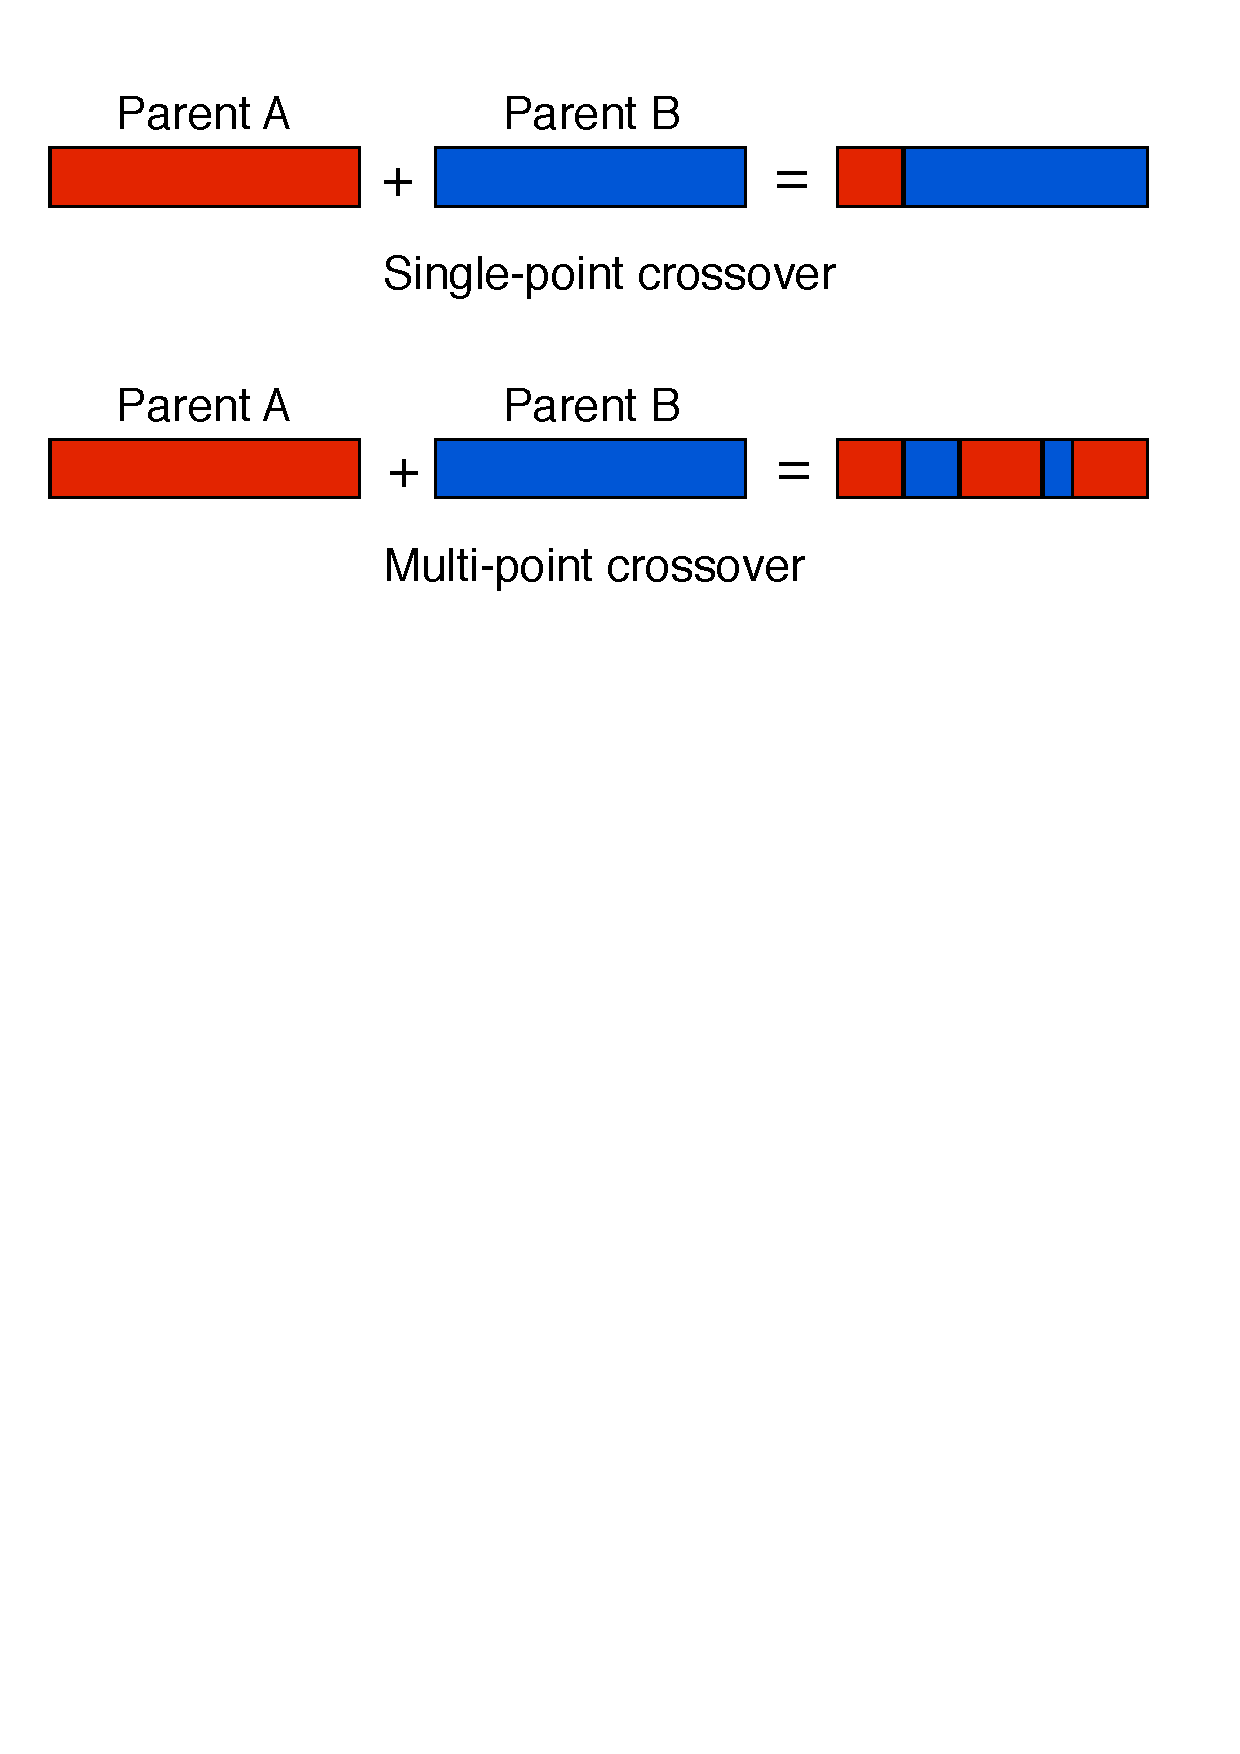
\includegraphics[width=0.7\textwidth,trim=0 18cm 0 0]{chapter_dalek/plots/crossovers.pdf} 
   \caption{In the single crossover a random point in the Individual is chosen. Before this point the genes are taken from the first parent and after that the we use the genes from the second parent. Using the same random number it easily allows for the creation of two children by reversing the roles of first and second parent. The multi-point crossover employs multiple places in the genome where the crossover happens.}
   \label{fig:crossover}
\end{figure}





\subsection{A simple example}
We will illustrate the use of a \ga\ on a simple astrophysical problem. The task at hand is to fit an observed spectrum with a synthetic spectrum. The input parameters for this synthetic spectrum are \teff, \logg, \feh, $\alpha$-enhancement, \vrad and \vrot. The simplest genetic representation of this is the vector $\vec{x} = (\teff, \logg, \feh, \alpha, \vrad, \vrot)$. $\vec{x}$ is the \textit{genotype} of the individual. The resulting synthetic spectrum is the \textit{phenotype}. 

For this relatively small number of genes a population size of 75 should suffice. The first step is drawing an initial population. We will draw uniformly randomly from the search space: $\teff \in [2000, 9000]$, $\logg \in [0, 5]$, $\feh \in [-5,1]$, $\alpha \in [0,0.4]$, $\vrad \in [-100, 100]$ and $\vrot \in [0,200]$. We compute the synthetic spectrum for each individual. The fitness of each individual is the inverse of the root-mean-square of the residuals between the observed and the synthetic spectrum. 
In the select step we will first advance 10 \% of the fittest individuals to the next population unaltered (\textit{elitism}). For the next population to be complete we need $75 - 8 = 67$ individuals which are created through mating. We select 2 individuals through \textit{roulette wheel selection} and place them in the mating pool. A single crossover point is randomly selected and the child is created. Before being placed in the new population the mutation operator is applied but has a very small chance to mutate any of the child's genes (in this case we choose 2\%).
This mating step (see Figure \ref{fig:example_mating}) is repeated 67 times. The new population now consists of the 8 fittest individuals of the old population and 67 new individuals created by mating. We will then start again to compute the synthetic spectrum and the resulting fitness for each individual of the new population. This loop is continued until one individual or a whole population has reached a preset convergence criterium.

\subsection{Convergence in Genetic Algorithms}
A key problem with many \ga-implementations is the premature convergence on a local optimum. The more complex the search space and the more interlinked the parameters are, the more likely it is that traditional search routines will fail. \ga s are inherently better at bypassing local optima but are in no way immune to this problem. A feature that separates \ga s from traditional optimization algorithms is that they will never fully converge. The algorithm will get close to the optimum but due to continued mutation of the individuals the \ga\ will in most cases not reach it. To alleviate this problem some authors suggest switching to a different algorithm when close to the optimum solution, whereas others suggest changing the mutation rate over time \citep[see][and references therein]{citeulike:344183}.
A definite advantage of \ga s is their parallel nature. Many other search algorithms require the evaluation of one solution to calculate the next step. The inherent parallel nature of \ga s makes it easy to explore large search spaces in the era of increasingly parallel computing. 

There are many advantages to using \ga s, however one of the unsolved problems is determining a mathematical description for their convergence. The predominate schemata theory explains only a subset of the intrinsic complexity of \ga s.

\subsection{GA theory schemata theory}

The schemata-theory first described by \cite{holland1975} is one of the accepted theoretical interpretations of \ga s. There is some criticism and it is known that this theory only explains part of the complexity that are inherent to \ga s \citep[see ][ and references therein]{Whitley94agenetic}. We will describe the basic concepts of schemata using an example in binary encoding \citep[notation adapted from ][]{citeulike:125978}. A schema or similarity template is formed by adding an extra letter to the binary alphabet denoted by $*$. Using the ternary alphabet ${0, 1, *}$ we can now describe a pattern matching schemata were the $*$ symbol can be thought of as \textit{don't care}-symbol. The schemata ${0, 1, 0, *}$ for example, matches both the string ${0, 1, 0, 0}$ and ${0, 1, 0, 1}$. The order of a schema is defined as how many places are not filled by the $*$-symbol. The given example is an third order schemata. Schematas provide a powerful way to describe similarities in a set of genomes. 
A whole population of solutions therefore samples a range of different schematas . Essentially low-order and above-average schemata receive exponentially increasing trials in subsequent generations of a \ga. \citet{Michalewicz:1994:GAD:184675} describe the workings of a \ga\ in the following way: ``A genetic algorithm seeks near optimal performance through the juxtaposition of low-order, high-performance schemata, called building blocks''.
This schemata-theory is the standard explanation for \ga s, there are however some examples that violate this \citep[see chapter 3 of][for some examples]{Michalewicz:1994:GAD:184675}.


\section{Genetic Algorithms to fit Type Ia Supernovae: The Dalek Code}
\label{sec:geneticdalek}

As described in Section \ref{sec:manual_sneia} the search-space for fitting \sneia\ is very complex and vast. The parameters that need to be fit are luminosity, photospheric velocity (\vph), Carbon, Magnesium ,Silicon, Sulfur, Calcium, Chromium, initial Ni ($\textrm{Ni}_0$) and primordial iron ($\textrm{Fe}_0$). As in the manual fitting example the time since explosion as well as the luminosity distance (for scaling purposes) are given. The evaluation for each spectrum takes roughly one minute on a modern computer which makes it hard to quickly try out different optimization strategies. We initially tried a Newton-Raphson approach with multiple phases. In the first phase the algorithm would adjust luminosity and normally came close to the optimum. In a second phase we tried to let the algorithm re-adjust luminosity, then photospheric velocity and last \ige s. This was modelled after the manual approach that is taken by \citet{hachinger_dipl2007} and \citep{hachinger_phd2011}. It took relatively long and would not converge. We realized quickly the search space is far to complicated for such simple methods. In addition, we were limited to one processor with this gradient method as the \mlc\ itself is not parallel. \ga s seem the perfect choice for this problem. They are easy to implement, can easily be parallelised and are relatively immune to local minima. 
For most of our optimization tests we worked with the supernova \sn{2002}{bo} \citep{2004MNRAS.348..261B}. This supernova is believed to be a ``Branch''-normal and is spectroscopically well sampled. For most of our tests we worked on the \texp=10.4 days spectrum, but did not make any other special assumptions about the spectrum. We have used some other spectra and will mention these where applicable.

\subsection{The Dalek Code}

After the failed attempts of the multi-phase Newton-Raphson fitter we launched straight into \ga s. As described in Section \ref{sec:ga_intro} one needs to first create an initial population. One can easily draw uniform randomly for luminosity and \vph (within some bounds). This method does not work for the elemental abundances as the sum of the abundances needs to add up to 1. For many normal supernovae the W7-abundances  \citep{1984ApJ...286..644N} give a good starting point. A population that is distributed around the optimum value converges mucg quicker than a uniformly sampled one. To calculate these abundances we need to know the photospheric velocity. Using data from \citet{2005ApJ...623.1011B} we have estimated an empirical relationship between the time since explosion and the photospheric velocity (see Figure \ref{fig:texp_vph}). This will serve as a rough first guess.

\begin{figure}[htbp] %  figure placement: here, top, bottom, or page
   \centering
   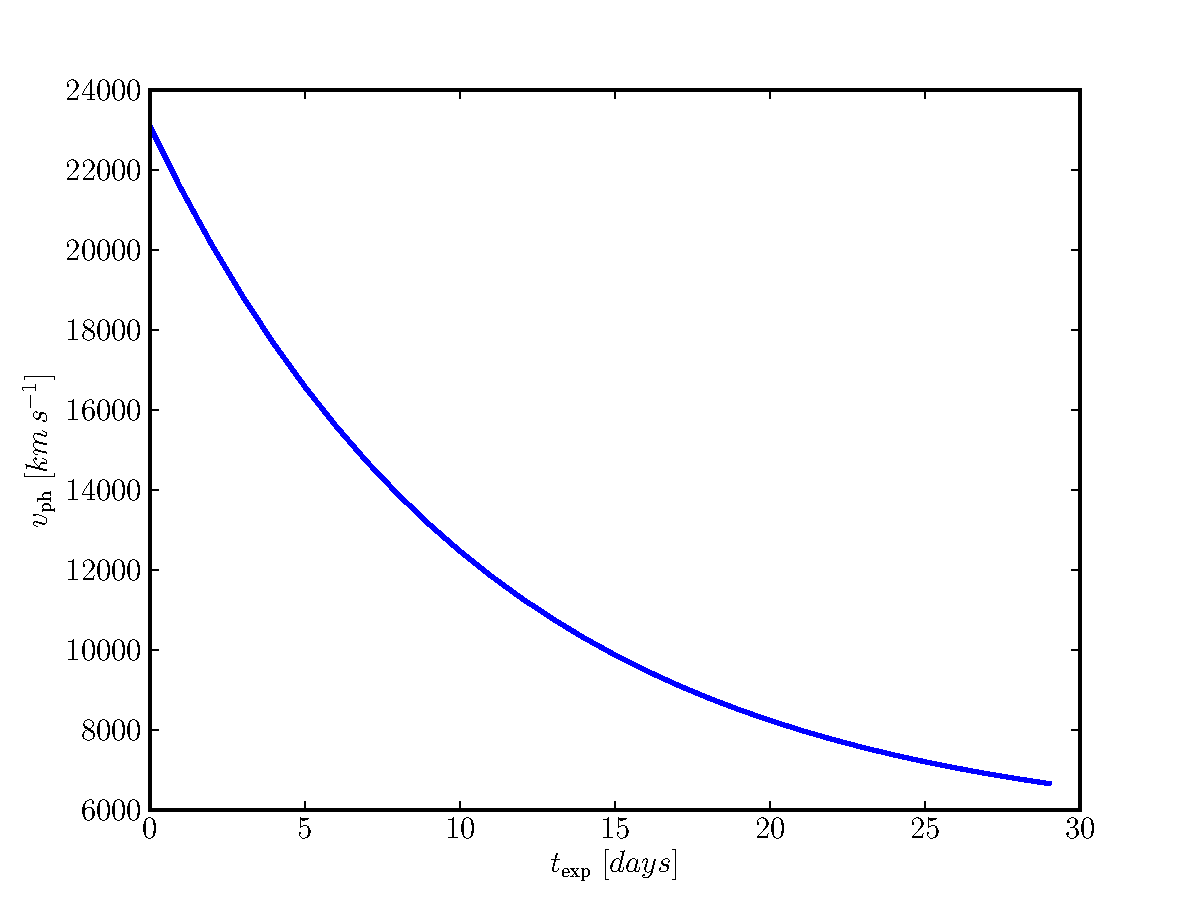
\includegraphics[width=0.7\textwidth]{chapter_dalek/plots/plot_texp_vph.pdf} 
   \caption{Estimated initial guess for photospheric velocity against days after explosion. }
   \label{fig:Intrinsic }
\end{figure} 

Once we know a \vph-estimate we can determine at what depth the photosphere is located in the W7-model. We use this point and integrate outwards to find our initial abundance fractions.

When creating our initial population we draw uniformly random for a preselected luminosity range (for the moment determined manually), a \vph-range 4000\,\kms above and below the \vph-estimate and asymmetric log-normal centered on the abundance estimate from W7. Creating the abundance values brings some problems with it. There are several bounds when it comes to the initial abundance ratios. We have a minimum bound for each abundance (established as the smallest abundance an element can have by \mlc) at $10^{-7}$ and a maximum bound which is determined by the requirements that all abundances need to add up to 1. If we would draw the abundances every time in the same order it would mean that the last element to be drawn would always have a very low chance of obtaining a high abundance value. Thus we randomize the order of drawing the elemental abundances.  Before we let an individual into the initial population we also check some abundance ratios by employing generous limits that we think are allowed by explosive nucleosynthesis of a \cowd \citep[e.g.][]{1999ApJS..125..439I}. 

\begin{itemize}
\item C $<$ 12.5\,\%
\item Si $>$ 1\,\%
\item Ca $<$ 5\,\%
\item Ti + Cr $<$ 1\,\%
\item $\textrm{Ni}_0$ $<$ 80\,\%
\item C $<$ O
\item 1 $<$ Si/S-ratio $<$ 10
\item Fe$_0$/Ni$_0$-ratio $<$ 10
\item Cr/Ni$_0$-ratio $<$ 10
\end{itemize}

If the newly created individual does not conform with these rules it is discarded and a new one is drawn. This process is repeated until we reach our population size which we chose to be 150.

Once the initial population is created it is distributed among the compute nodes by the \dalek. As we need to explore a large parameter space we use a distributed computing approach. The scheduler part of \dalek\ distributes parameter sets to spectrum synthesizers working on different machines across the network. The difficulty is (and the reason that we didn't use a standard implementation like MPI) that we need the \dalek\ to reach processors on many different architectures and operating systems. This enables us to harness a large fraction of the institutes computational power. For the order of execution we have chosen a very simple scheduling algorithm that maintains a FiFo batch-queue for the parameter sets and distributes them among the pool of spectrum synthesizers.

The resulting spectra are then subjected to a fitness function. The determination of the fitness function is one of the most crucial  choices for the \ga\ to work. The correct fitness function is still a field of active research in the \dalek. As an initial approach we calculated the mean-square of the residuals remaining from subtracting the observed spectrum and the spectrum of the current individual. This approach has two main issues: For almost all observed spectra in the early phase the fitted spectrum has a large continuum excess beyond 6500 \AA (see Figure \ref{fig:sn2002bo-10_bf}). We still regard the line depth and line shape to be correct. As described previously this is a known issue of the \mlc. This large difference in the infrared means that the \dalek\ will try to optimize this large offset and pay less regard to a good fit in the rest of the spectrum. To alleviate this we have tried multiple approaches. At first we tried to de-weight the fit in the problematic region. This artificially introduced weighting factor introduces another parameter which might have to change it for the \ga\ to succeed on different spectra. This would defeat the point of an automatic fit. As a second approach we tried to fit and subtract the continuum in the problematic region before creating our fitness figure. 
In addition, the \mlc\ supllies us with an estimate of the dilution factor W at the photosphere. This factor is expected to be close to 0.5 (see description in \ref{sec:mlc_code}). \citet{hachinger_dipl2007} and \citet{hachinger_phd2011} have found that in all cases a good fit will have a value of the dilution factor between 0.4 and 0.7. We have incorporated this into the fitness calculation and de-weight spectra with a value outside this range to a great extent.
We should mention that we have tried, in addition to calculating the root-mean-square of the spectra, a number of different methods. Most notably we tried to use neural-networks to perform a goodness of fit analysis. We however abandoned this effort as the training set to calibrate neural networks requires a large number of well fitted spectra which are not available. 

Once the fitness is calculated for each individual we use the method of fitness scaling to preempt premature convergence in early generations (caused by the so called ``super-individuals'') as well as creating a steeper fitness gradient in later generations. We have decided to use a linear fitness scaling as described in \citet{citeulike:125978}:
\[
f^\prime = af+b,
\]
where $f\prime$ designates the scaled fitness and $f$ the raw fitness.
In all cases we want to make sure that the average of the scaled fitness $f_\textrm{avg}^\prime$ equals that of the average of the raw fitness $f_\textrm{avg}$. We will first try to find a linear relation so that the new maximum fitness $f'_\textrm{max}$ is $C_\textrm{mult}$ times the average fitness ($f_\textrm{avg}$). We choose $C_\textrm{mult}=2$ as suggested by \citet{citeulike:125978}. This operation will scale early ``super-individuals'' down and the rest of the population up and preempts premature convergence. In the later phases of the \ga, when the fittest individuals and the bulk of the population have similar fitness values, this operation would lead to negative fitnesses for some individuals. In that case we find scaling parameters that maps the least fit individual to a fitness value of 0, while still maintaining $f_\textrm{avg}^\prime=f_\textrm{avg}$. Once we have scaled the fitnesses we move to the selection process.

In the current version of the \dalek\ we employ \textit{elitism} (10\% of fittest individual advance immediately to next generation). We have also experimented with other modifications to the mating population, but found them to be subpar. The mating pool we have chosen has only two slots. For now we select the individuals for the mating pool using the standard \textit{roulette wheel selection}. We use a crossover probability of 90\%, this means that in 10\% of the cases we do not perform crossover but the child is a copy of the first parent. If crossover occurs, we perform a uniform crossover as we felt that we do not want the ordering of the parameters to matter. We have also experimented with arithmetic crossovers by taking the mean of parents. This meant that often useful traits would entirely disappear and we switched back to uniform crossovers. We will experiment in the near future with different crossover techniques like single-point crossovers. The new individual, created by crossover, is subjected to possible mutations before being placed into the new population. The \dalek\ employs different mutation strategies for the different parameters. The abundances are just multiplied by a uniform random number (we have tried gaussian random numbers) with a relatively high chance of currently 7\%. As luminosity and photospheric velocity are physically different we treat them differently to the abundances. In both cases we add a uniform random number, in addition to having different mutation probabilities. After the mutation step we see if the buffer element oxygen has a negative abundance. A negative abundance implies that the other elements add up to more than 1. If oxygen has positive abundance the code goes on to check the abundance ratios. If the child passes both these tests it is placed in the new population, if not it is discarded. This process is repeated until the size of the new population (including the members of the old population that advanced through \textit{elitism}) reaches 150.

This process of selection, recombination and mutation is repeated over many generations. We have experimented with up to a 1000 populations in one run. Our scheduler can achieve a throughput of one generation per minute (in optimal conditions where all CPUs are free). 
Our principal spectrum for the testing was \sn{2002}{bo} 10.4 days post explosion (see Figure \ref{fig:sn2002bo-10_bf}). 
In the presented case we let the \ga\ run for 188 generations. Figure \ref{fig:fitness_evolution} shows how the genetic algorithm over many generations improves the fitness of the indivduals. 

\begin{figure}[htbp] %  figure placement: here, top, bottom, or page
   \centering
   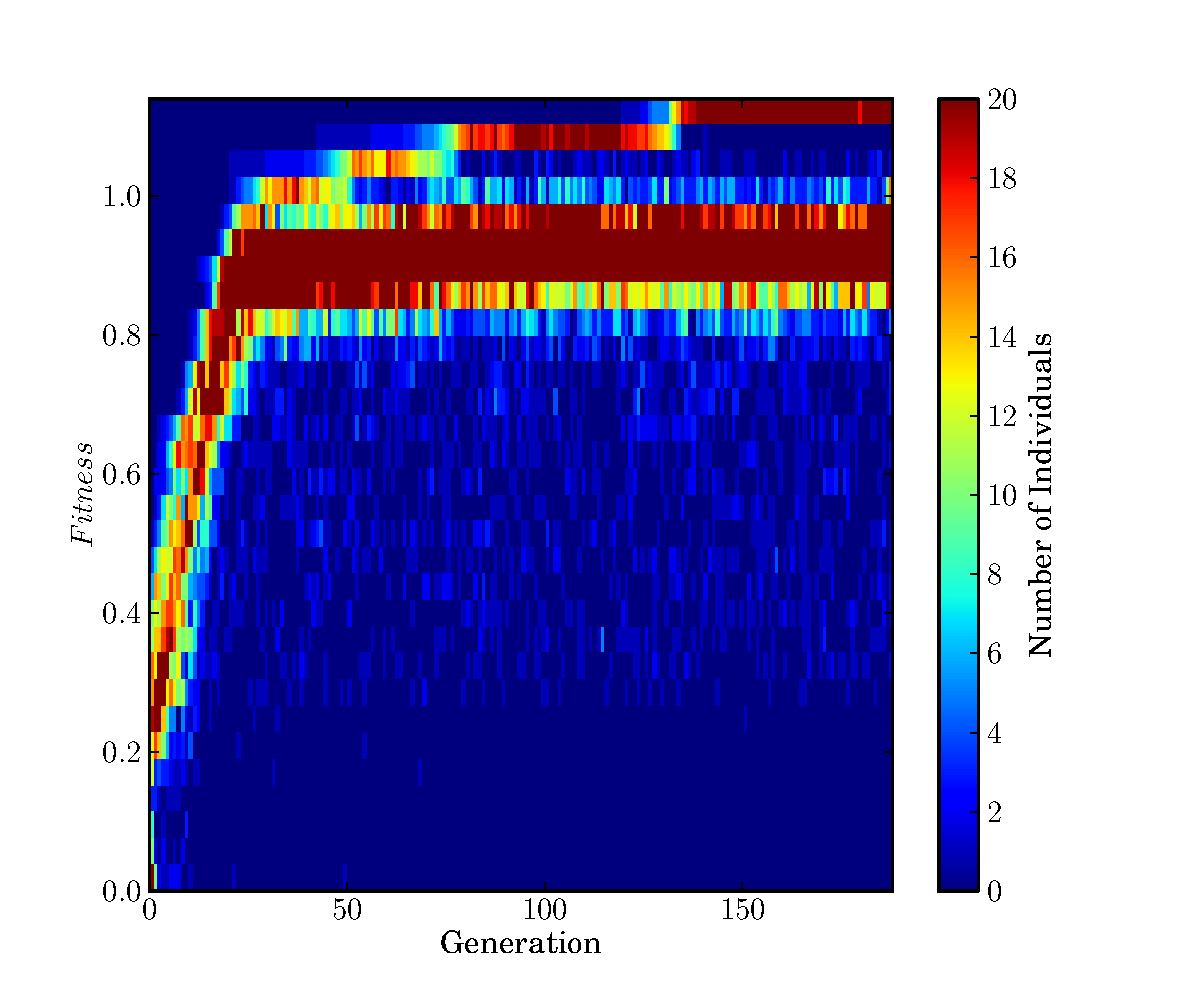
\includegraphics[width=0.7\textwidth]{chapter_dalek/plots/plot_02bo_fit_evol.pdf} 
     \caption{Evolution of fitness of in the generations. In later generations there is a clear divide between the members that have advanced through elitism and the bulk of the population. This suggests a too high mutationrate or the convergence of the algorithm. }
   \label{fig:fitness_evolution}
\end{figure}

The step-pattern is very common in genetic algorithms: One individual has a favorable mutation and it takes several generations for the others to catch up. During the last generations one can clearly see that there is a gap between bulk of the population is and the top 10\%. This gap is caused by the contrast of relatively high mutation in the main individuals against the mutation free advancement of the top 10\% (\textit{elitism}).


\begin{figure}[htbp] %  figure placement: here, top, bottom, or page
   \centering
   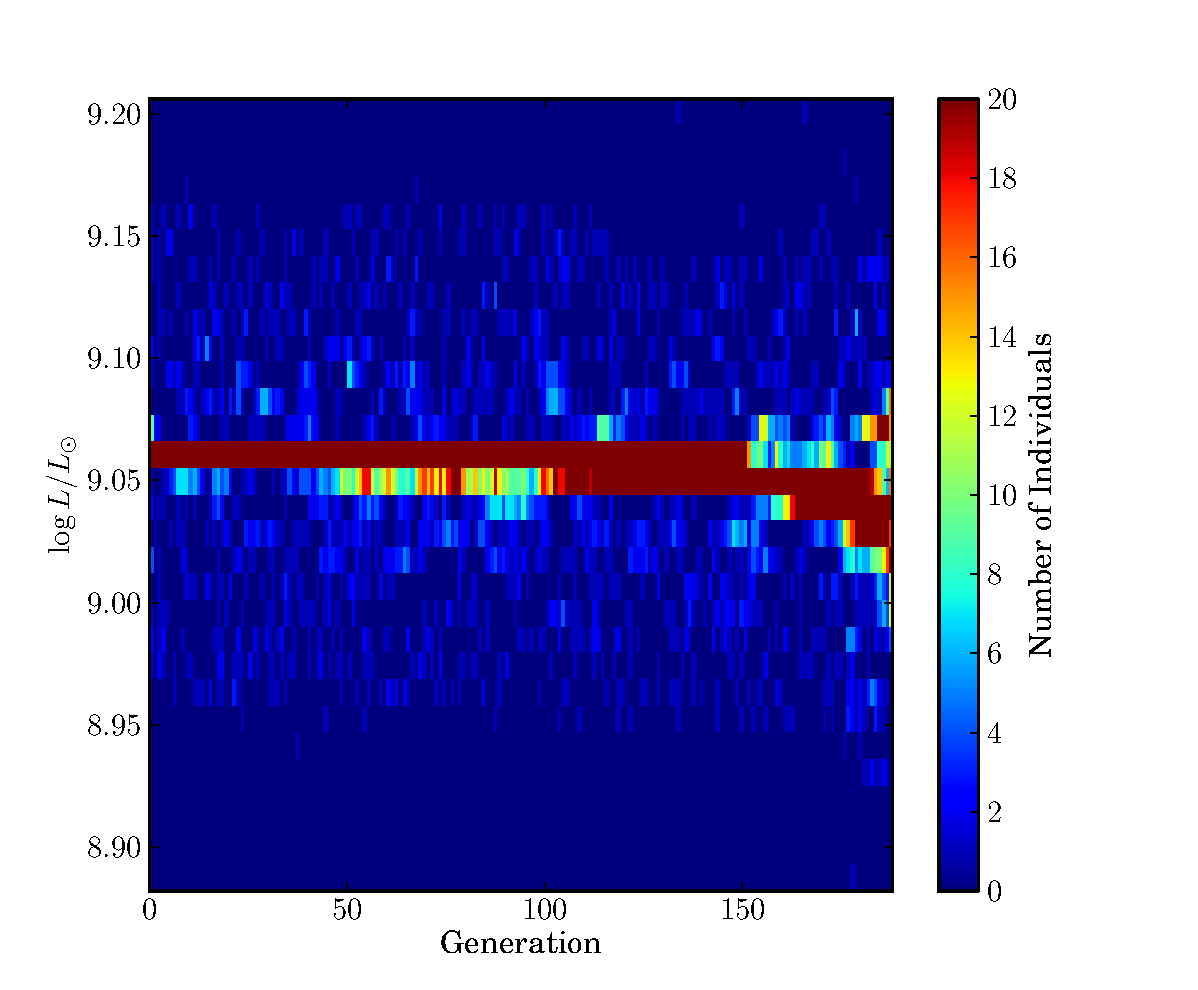
\includegraphics[width=0.49\textwidth]{chapter_dalek/plots/plot_02bo_lum_evol.pdf} 
   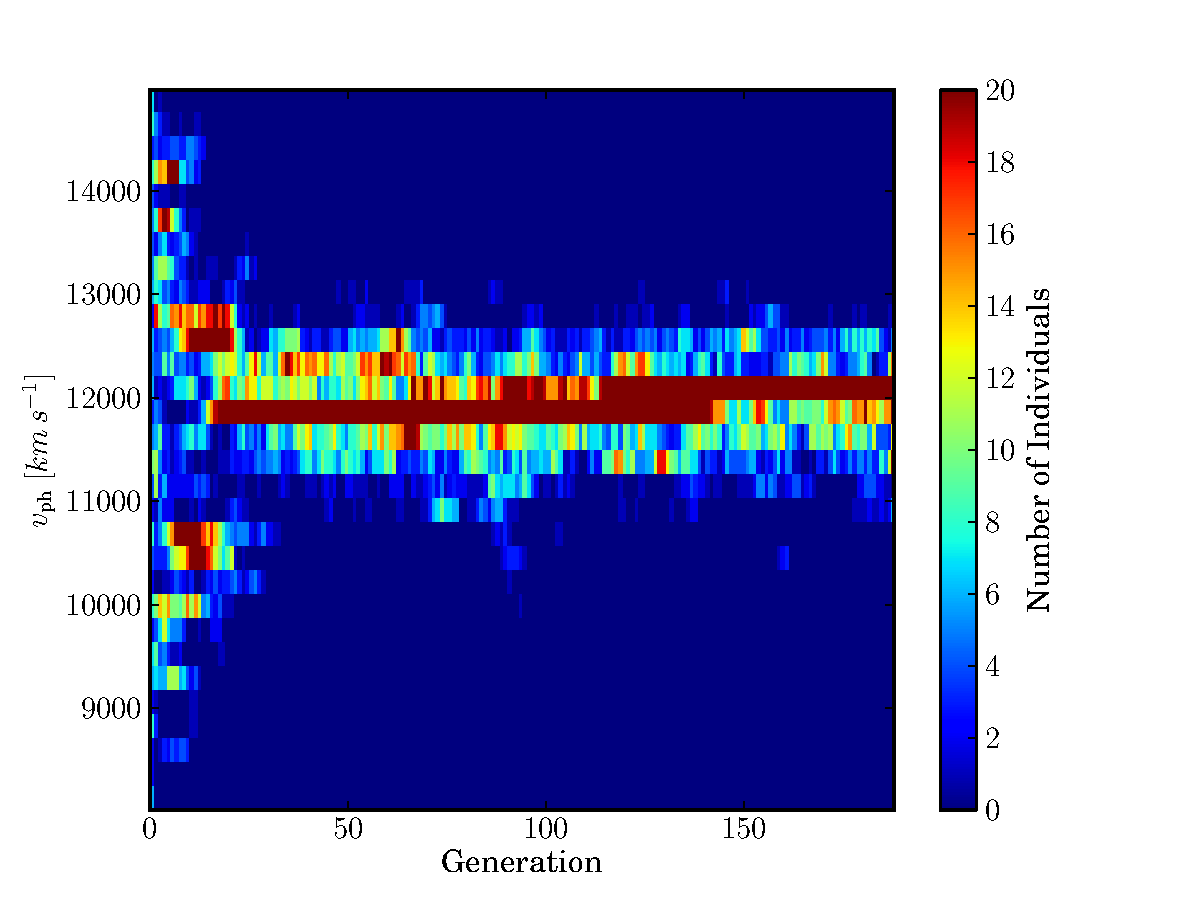
\includegraphics[width=0.49\textwidth]{chapter_dalek/plots/plot_02bo_vph_evol.pdf} 
   \caption{The evolution of both luminosity and photospheric velocity shows that even at late phases of the algorithm there are still new combination that are being trialled. The very quick convergence in both cases however is a bit worrisome and will be analysed in future experiments.}
   \label{fig:lumvph_evolution}
\end{figure}


Figure \ref{fig:lumvph_evolution} gives a good overview of how the genetic algorithm process through the search space. In our example the algorithm converges relatively fast (after roughly 30 generations). Even though there is a ``main''-population the algorithm still tries out different combinations. Currently we still have the problem that for certain initial random seeds the algorithm does not find the global optimum but converges prematurely on a local optimum. We believe the quick convergence seen in Figure \ref{fig:lumvph_evolution} might be evidence for this. This again is an area of active research and two experts in evolutionary optimization joined our team recently to address this problem. 

\begin{figure}[htbp] %  figure placement: here, top, bottom, or page
   \centering
   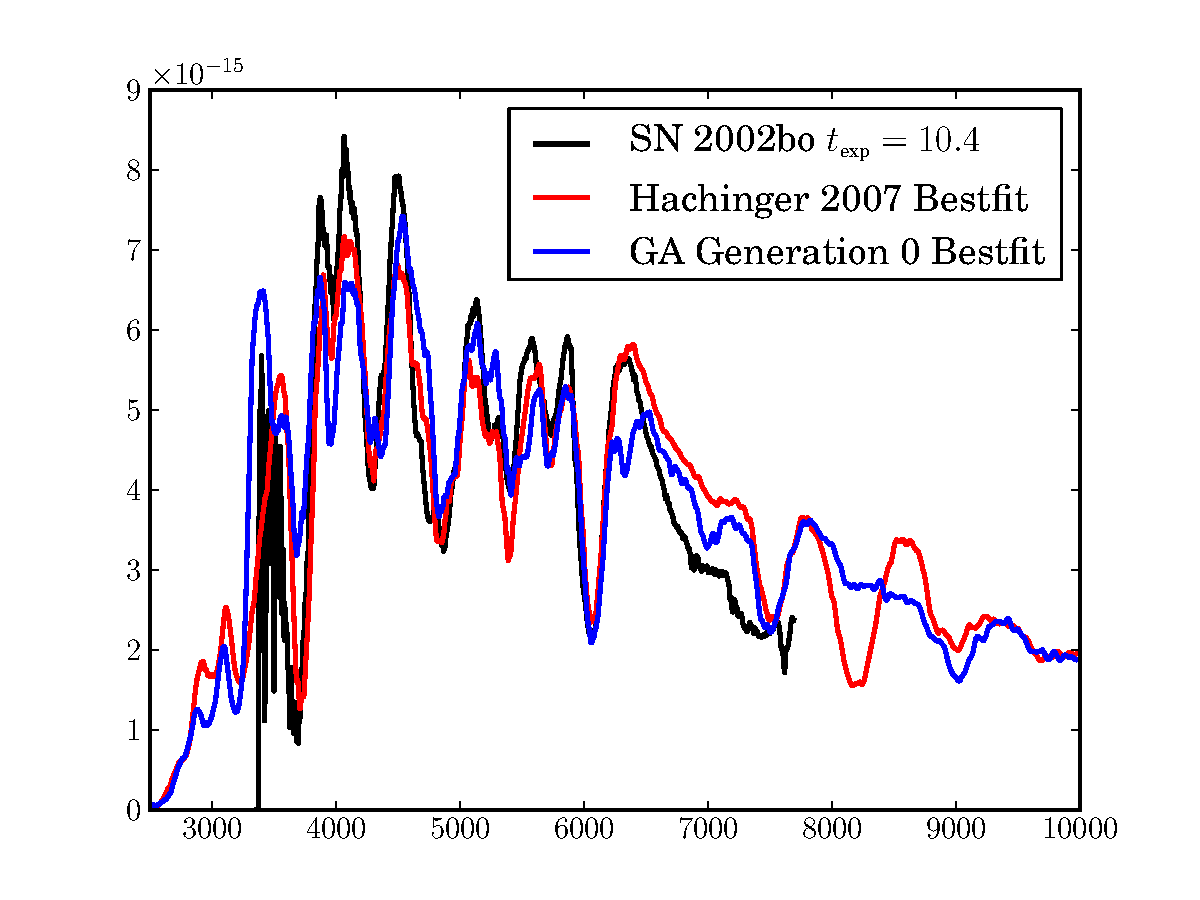
\includegraphics[width=0.49\textwidth]{chapter_dalek/plots/plot_ga0_speccompare.pdf} 
   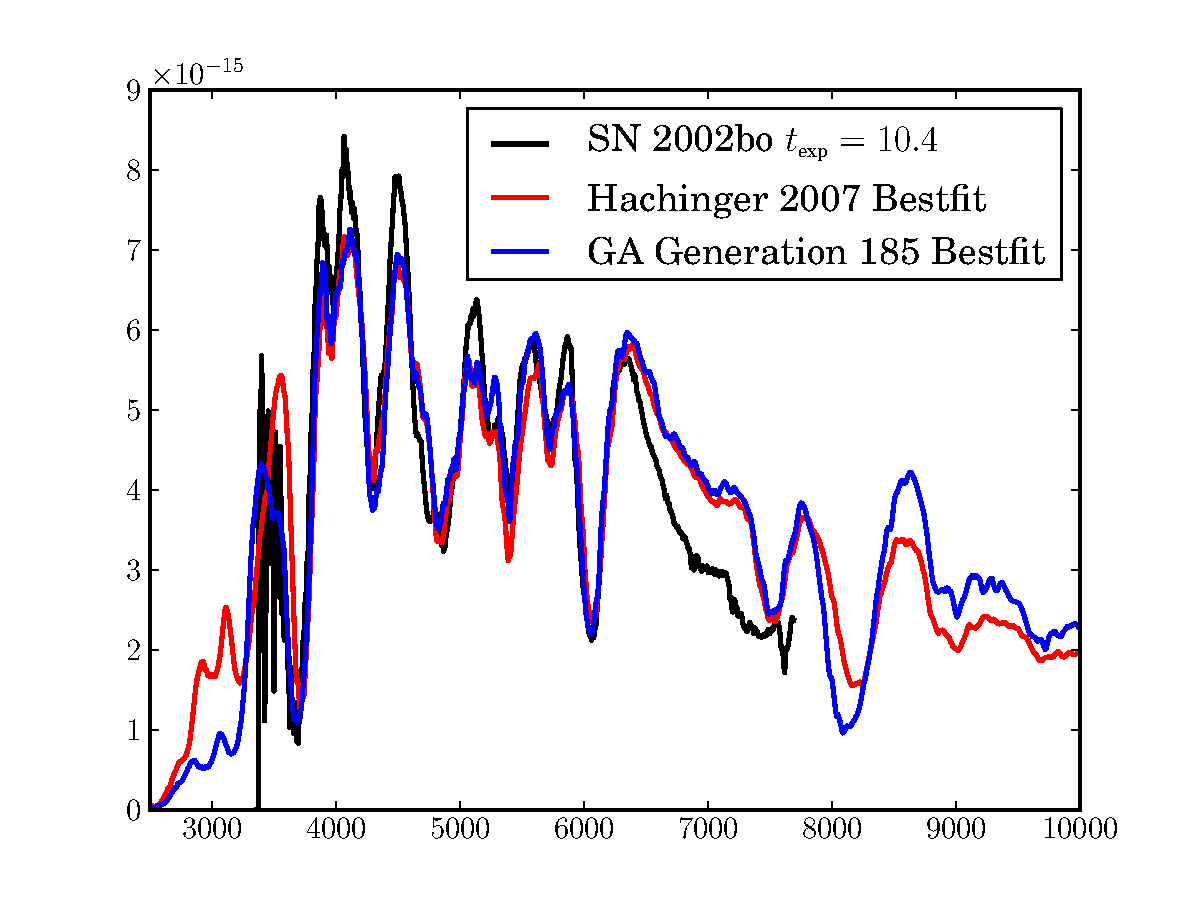
\includegraphics[width=0.49\textwidth]{chapter_dalek/plots/plot_ga185_speccompare.pdf} 
   \caption{The best individual of the first generation (left) and the best individual after 185 generations (right). This initial result demonstrates that \ga s are able to conquer this problem. A more stable convergence and thorough exploration of the parameter space is however necessary to use this technique on a set of supernova spectra.}
   \label{fig:example}
\end{figure}

Although there are still many outstanding problems we can show that the \ga s are able to solve the \sneia\ fitting problem. In Figure \ref{fig:ga_fit} we show the best fit in the first generation as well as the best-fit in the last generation. As comparison we show the best fit obtained by \citet{hachinger_dipl2007}. The \ga\ has been successful in reproducing the main features of the \sneia-spectrum. The de-weighting in the infrared is working very well. We are currently trialing the current code on different spectra with mixed results. 


\section{Conclusion}
\label{sec:dalek_conclusion}
\ga s are powerful tools, which can easily search a vast parameter space in parallel and avoid local optima. The intrinsic parallel structure has been a tremendous advantage in our experiments. We have shown that \ga s can successfully solve the problem and fit a \sneia-spectrum. We do acknowledge that our current implementation does not reliably work on all spectra and there remains lots of fine-tuning work to be done. This tweaking is very common in \ga\ implementations, but often requires experts in numerical optimization for speedy advancement. James Turner and Irene Mosner are experts in evolutionary optimization (their research focuses on differential evolutionary algorithms) and are currently exploring with our help the search space. 
On a different front we are currently exploring to optimize the exploration speed. Even on current high-end machines the \mlc\ takes one minute per synthetic spectrum per CPU. One of the ideas is creating a parameter grid around all or some of our search area. We could then use fast and efficient interpolation techniques (one of these is described in Chapter \ref{chap:ndinterp}) and explore different settings for our genetic algorithm much more quickly.

Over the course of this project we have realized that the field of numerical optimization has made huge strides in the last decades. Most of the new algorithms are not well known in astronomy and are used even rarer. On the other hand experts in the field of numerical optimization are often in desperate need for ``real world'' applications. They are more than willing to apply their knowledge to problems in our field. We strongly believe that there is an important ground for collaboration that would benefit both sides immensely.





